\documentclass[12pt,a4paper,oneside]{book}
\usepackage[top=3cm, bottom=3cm]{geometry}
\usepackage[utf8]{inputenc}
\usepackage[spanish]{babel}
\usepackage[toc,page]{appendix}
\usepackage{longtable}
\usepackage{amsmath}
\usepackage{amsfonts}
\usepackage{float}
\usepackage{amssymb}
\usepackage{listingsutf8}
\usepackage{color, soul}
\usepackage{paracol}
\usepackage{listings}
\usepackage{listingsutf8}
\usepackage{verbatim}



\def\CS#1{\texttt{\textbackslash#1}}

\usepackage[most]{tcolorbox}

% Para escribir comandos como linea de comando 
\newtcblisting{commandshell}{colback=black,colupper=white,colframe=black!75!black,listing only,listing options={style=tcblatex,language=sh},every listing line={\textcolor{white}{\small\ttfamily\bfseries control \$> }}}

\newtcblisting{dns}{colback=black,colupper=white,colframe=black!75!black,listing only,listing options={style=tcblatex,language=sh},every listing line={\textcolor{white}{\small\ttfamily\bfseries dns \$> }}}

\newtcblisting{origin}{colback=black,colupper=white,colframe=black!75!black,listing only,listing options={style=tcblatex,language=sh},every listing line={\textcolor{white}{\small\ttfamily\bfseries origin \$> }}}

\newtcblisting{frontend}{colback=black,colupper=white,colframe=black!75!black,listing only,listing options={style=tcblatex,language=sh},every listing line={\textcolor{white}{\small\ttfamily\bfseries frontend \$> }}}

\newtcblisting{backend}{colback=black,colupper=white,colframe=black!75!black,listing only,listing options={style=tcblatex,language=sh},every listing line={\textcolor{white}{\small\ttfamily\bfseries backend \$> }}}

\newtcblisting{logs}{colback=black,colupper=white,colframe=black!75!black,listing only,listing options={style=tcblatex,language=sh},every listing line={\textcolor{white}{\small\ttfamily\bfseries}}}


% Para escribir script o parte de ellos
\usepackage{lipsum}
\usepackage[T1]{fontenc}
\definecolor{gray90}{gray}{.90}
\lstdefinestyle{codigobase}{
basicstyle=\small\ttfamily,
frame=single,
backgroundcolor=\color{gray90},
}

%%%%%%%%%%%%% Macros para formato 302 %%%%%%%%%%%%%%%%%%%

% Metadata para el PDF a generar 
\usepackage[unicode,
            pdftex]{hyperref}
\hypersetup{
 pdfauthor={Lucas Viera - 177863, Bruno Riccardi - 185531},
 pdftitle={Sistema de Distribución Multicast mediante Redes Definidas por Software.},
 pdfsubject={SHERMAN: Una red virtual para la distribución de contenido},
 pdfkeywords={completar, palabras, clave}
 }

% Numeración y formato de páginas
\usepackage{fancyhdr}
\pagestyle{fancy}
\fancyhf{}
%\fancyhead[lo,le]{\nouppercase{\rightmark}}
\fancyfoot[RO]{\thepage}

\fancypagestyle{plain}{
  \fancyhf{} 
  \fancyfoot[RO]{\thepage}
  \renewcommand{\headrulewidth}{0pt}}
\renewcommand{\headrulewidth}{0pt}


% Indice (estos parámetros se pueden cambiar)
\setcounter{secnumdepth}{3} %para que ponga 1.1.1.1 en subsubsecciones
\setcounter{tocdepth}{3} % para que ponga subsubsecciones en el indice

%% Para incluir imagenes
\usepackage{graphicx}


% Para incluir tablas en español
\renewcommand\tablename{\bfseries Tabla}

% Para incluir listings de código
\renewcommand{\lstlistingname}{\bfseries C\'odigo}

% Para agregar la bibliografía al indice
\usepackage[nottoc,numbib]{tocbibind}


%%%%%%%%%%%%%%%%%%%%%%%%%%%%%%%%%%%%%%%%%%%%%%%%%%%%%%

% Generación del índice
\makeindex


% Empieza el documento
\begin{document}
% Portada 

\begin{center}
\thispagestyle{empty}

\begin{Large}
\textbf{Universidad ORT Uruguay}

\textbf{Facultad de Ingeniería}
\vspace{4cm}
\end{Large}


\begin{huge}
\textbf{Sistema de Distribucion Multicast mediante Redes Definidas por Software} 

\end{huge}

\vspace{2cm}

\textbf{Entregado como requisito para la obtención del título de Ingeniero en Telecomunicaciones}

\vspace{5cm}

\begin{large}
\textbf{Lucas Viera  - 177863.}\\
\textbf{Bruno Riccardi - 183531.}\\
\bigskip

\textbf{Tutor: Álvaro Sanchez}
\vspace{2cm}
\end{large}

\begin{huge}
\textbf{2019}
\end{huge}

\end{center}



\chapter*{Declaración de autoría}



Nosotros, Bruno Riccardi y Lucas Viera, declaramos que el trabajo que se presenta en esta obra es de nuestra
propia mano. Podemos asegurar que:
\begin{itemize}
\item La obra fue producida en su totalidad mientras realizábamos el proyecto de fin de carrera;
\item Cuando hemos consultado el trabajo publicado por otros, lo hemos atribuido con claridad;
\item Cuando hemos citado obras de otros, hemos indicado las fuentes. Con excepción de estas citas, la obra es enteramente nuestra;
\item En la obra, hemos acusado recibo de las ayudas recibidas;
\item Cuando la obra se basa en trabajo realizado conjuntamente con otros, hemos explicado claramente qué fue contribuido por otros, y qué fue contribuido por nosotros;
\item Ninguna parte de este trabajo ha sido publicada previamente a su entrega, excepto donde se han realizado las aclaraciones correspondientes.
\end{itemize}

 
\vspace{2cm}


\includegraphics[scale=0.08]{fotos/0_Caratula/firmas/firmaLucasBYN.JPG} \hfill

\includegraphics[scale=0.08]{fotos/0_Caratula/firmas/firmaBrunoBYN.JPG} \hfill


Lucas Viera CENTRAR y poner fecha del dia . \hfill  Bruno Riccardi \\

\vspace{1cm}


{\centering 01/08/2019 
 
}


\chapter*{Abstract}

El resumen debería permitir comprender rápidamente:

- Cuál es el tema, problema o situación analizada

- Por qué tiene interés o relevancia

- Qué se hizo en el trabajo (métodos y procedimientos) – lo que se analizó, produjo o estudió y de qué manera.

- Qué resultados se obtuvieron de dicho trabajo

- Qué conclusiones se extraen de los resultados



\vspace{0.5 cm}

Debe considerarse como un documento independiente, que en muchos casos circula por separado del trabajo final. Muchas bases bibliográficas utilizan el resumen como herramienta fundamental (o incluso única) de despliegue de resultados, para que el lector decida si desea acceder al contenido completo; a menudo, las decisiones iniciales de aceptación de trabajos a conferencias se realizan a partir del resumen.

\vspace{0.5 cm}
1. Sigue la estructura básica indicada: problema o tema estudiado, justificación y relevancia, métodos y procedimientos, resultados y conclusiones (o, alternativamente, la estructura especificada por la cátedra para el tipo específico de trabajo).

2. El contenido del abstract es consistente con el del trabajo. Utiliza los términos o palabras clave correspondientes al contenido del trabajo.

3. Resume toda la información sustancial del trabajo, incluyendo en particular los métodos y conclusiones.

4. No contiene términos vagos o indefinidos, ni omite aspectos importantes del trabajo.

5. Se ajusta a la extensión máxima indicada en el documento de formato.


\vspace{0.5 cm}
Consiste de un resumen del contenido del trabajo, que se usa para difusión y para que el lector potencial sepa en qué consiste el trabajo sin necesidad de leerlo completamente. Puede tener una extensión máxima de 400 palabras. Debe existir coherencia entre el contenido del trabajo final y el abstract. Ver documento 306 (Orientación para títulos, resúmenes o abstracts e informes de corrección de trabajos finales de carrera)

% % Durante los últimos años las redes de distribución de contenido han jugado un rol decisivo en la evolución que ha tenido Internet hacia redes multimedia, tendencia que se mantendrá a futuro\cite{cisco2019}. Por otro lado, la búsqueda de virtualizar funciones con el objetivo de mejorar los rendimientos y aprovechar mejor los recursos ha incrementado. En ese ámbito es que se desarrolla esta tesis.

% \vspace{0.5cm}

% La motivación surge ante la inquietud de encontrar técnicas para enfrentar la fuerte variación en la demanda de actividad por parte de los usuarios en sistemas de streaming de video. Esto ha hecho que surjan nuevas formas de gestionar los recursos de sistemas de información, que ya no deben dimensionarse a su máxima capacidad de usuarios\cite{servidor_de_streaming_cdn}.

% \vspace{0.5cm}

% Se logró diseñar e implementar una red virtual de distribución de contenido para Video on Demand enfocada en el automatismo de funciones como son el caché y la adaptación de infraestructura en función de la demanda de los usuarios.

% Además, ésta cumple los planteamientos definidos por el modelo ETSI-MANO, lo cual brinda la valiosa capacidad de integrarse con otros componentes que sigan el mismo estándar. 

% \vspace{0.5cm}

% Todo el desarrollo fue realizado utilizando únicamente herramientas de software libre. Se destacan entre ellas OpenStack, el núcleo de este proyecto, Apache Traffic Server como componente fundamental de las funciones de vCDN, junto con Django y Ansible para la completa integración.

% Se desarrolló un sistema de enrutamiento para las peticiones de los usuarios basado en zonas DNS, permitiendo brindar el contenido de forma inteligente desde el punto más adecuado de la red.

% \vspace{0.5cm}

% El sistema cuenta con interfaces amigables para la interacción con los usuarios. Entre las principales funcionalidades se encuentran la gestión y monitoreo de recursos, el manejo de políticas de caché, almacenamiento y la reproducción de videos con streaming adaptativo.

% \vspace{0.5cm}

% Con los resultados obtenidos se puede afirmar que el proyecto fue exitoso. Más allá de los objetivos cumplidos, el desarrollo fue un gran proceso de aprendizaje. Durante el mismo se investigaron y utilizaron muchas tecnologías que no forman parte del plan de estudios de la carrera, lo cual aportó una enriquecedora experiencia en temáticas que están teniendo una gran repercusión en el mundo actual. 


\chapter*{Palabras clave}

API: Application Programming Interface (Interfaz de programación de aplicaciones). Es el conjunto de herramientas de software que presenta un determinado programa o aplicación para que otros accedan a él y lo puedan utilizar como abstracción.

\vspace{0,5cm}

ARP: Address Resolution Protocol (Protocolo de resolución de direcciones). Es un protocolo que se encarga de traducir una dirección IP de capa de red a una dirección MAC de capa de enlace.

\vspace{0,5cm}

Broadcast: 
método de transmisión de datos en redes de área local que envía el tráfico desde un nodo de origen a todos los demás.

\vspace{0,5cm}

Datacenter: 
un datacenter o centro de datos es un repositorio centralizado de información, formado por varios equipos reales y/o virtuales interconectados.

\vspace{0,5cm}

Datapath: en SDN, un datapath es la representación lógica de un equipo de red que presenta acceso a un conjunto de recursos de red, así estos estén distribuidos en varios equipos reales. Cada datapath está identificado unívocamente por un DPID (Datapath ID), un número hexadecimal de 8 bytes.

\vspace{0,5cm}

Dirección MAC: la dirección de control de acceso al medio (Media Access Control) es una dirección asignada a un equipo físico por la lógica de la capa de enlace y está compuesta por 6 octetos (6 bytes). Habitualmente se expresa en formato hexadecimal de forma XX:XX:XX:XX:XX:XX.

\vspace{0,5cm}

Host: un equipo conectado a la red como cliente, ya sea un servidor, un PC o cualquier equipo que transmita y/o reciba datos.

\vspace{0,5cm}

ICMP: Internet Control Message Protocol (Protocolo de Mensajes de Control de Internet) es un sub protocolo del protocolo de Internet (IP) que entre otros servicios, provee la posibilidad de enviar paquetes de “echo”, que son utilizados por los comandos “ping” y “traceroute”.

\vspace{0,5cm}

ISP: Internet Service Provider (Proveedor de Servicios de Internet). Es una empresa que brinda servicios de Internet a sus clientes. Por ejemplo Antel.

\vspace{0,5cm}

IGMP:

\vspace{0,5cm}

JSON: JavaScript Object Notation (Notación de objetos de JavaScript). Es un formato liviano para el intercambio de datos, que resulta fácil de leer para los seres humanos y de interpretar y generar para las máquinas.

\vspace{0,5cm}

Latencia: la suma de retardos temporales en una red. En muchos casos se ha considerado como latencia el retardo temporal de ida y vuelta de un paquete.

\vspace{0,5cm}

Mininet: Simulador de red que corre en sistemas operativos Unix y permite simular redes con varios switches en diferentes topologías y los hosts conectados a ellos.

\vspace{0,5cm}

Multicast: método de transmisión de datos en redes de área local que envía el tráfico desde un nodo de origen a un grupo de los demás nodos. Esto se logra utilizando una dirección de destino (IP o MAC) de un rango reservado.

\vspace{0,5cm}

Network Function Virtualization.

\vspace{0,5cm}

OpenFlow:protocolo diseñado para la comunicación entre el controlador y los switches 

\vspace{0,5cm}

OpenFlow en SDN.

\vspace{0,5cm}

Open vSwitch:

\vspace{0,5cm}

PIM:

\vspace{0,5cm}

Python: lenguaje de programación interpretado.

\vspace{0,5cm}

REST: Representational State Transfer (Transferencia de estado representativo) refiere a una interfaz entre sistemas que utiliza el protocolo HTTP para obtener datos o indicar la ejecución de operaciones sobre los datos.

\vspace{0,5cm}

RYU:

\vspace{0,5cm}

SDN: Software Defined Networks (Redes definidas por Software). Es un paradigma de redes de datos que propone la centralización del control de una red y su desacople del plano de datos.

\vspace{0,5cm}

Switch: en una red tradicional, un switch es un conmutador que trabaja con paquetes de datos a nivel de capa de enlace del modelo OSI. En una red SDN, un switch es un equipo que puede ser configurado por el controlador utilizando un protocolo, como OpenFlow, y tiene una mayor cantidad de funcionalidades disponibles.

\vspace{0,5cm}

Streaming:

\vspace{0,5cm}

Tabla de flujos: elemento fundamental de un switch OpenFlow. En esta tabla es donde se escriben las entradas o reglas de flujo.

\vspace{0,5cm}

Tabla de grupos:

\vspace{0,5cm}

Tráfico: paquetes de datos que atraviesan una red y son encaminados por los elementos de la misma.

\vspace{0,5cm}

Topología:

\vspace{0,5cm}

Trunk: puerto de interconexión entre dos switches donde se produce el etiquetado de las tramas.

\vspace{0,5cm}

Unicast: método de transmisión de datos en redes de área local que envía el tráfico desde un nodo de origen a un nodo de destino, identificado con una dirección IP y una dirección MAC.

\vspace{0,5cm}

VLAN: subred lógica a la que pertenecen uno o varios hosts de uno o varios segmentos de red de área local.

\vspace{1cm}

Conjunto de palabras que están directamente relacionadas con el contenido de la obra que además deberán ser incluidas en las
propiedades del archivo PDF para facilitar que el documento sea indexado por los buscadores.

% Content Delivery Network.



% \vspace{0.5cm}
% Virtual Content Delivery Netwrok.

%El siguiente comando genera el índice (no tocar)
\tableofcontents

\chapter{Introducción} 
\label{intro} % para poder referenciarlo después usando \ref{intro}

A modo de ejemplo introducimos el siguiente texto autogenerado:



Ejemplo de lista utilizando itemize:
\begin{itemize}
    \item Primero
    \item Segundo
    \item Tercero\\
\end{itemize}

Ejemplo de enumeración utilizando enumerate:
\begin{enumerate}
    \item Primero
    \item Segundo
    \item Tercero\\
\end{enumerate}

Ejemplo de enumeración anidada utilizando enumerate:
\begin{enumerate}
    \item Primero 
        \begin{enumerate}
        \item Primero
        \item Segundo
        \item Tercero
        \end{enumerate}
    \item Segundo
        \begin{enumerate}
        \item Primero
            \begin{enumerate}
            \item Primero
            \item Segundo
            \end{enumerate}
        \item Segundo
        \end{enumerate}
\end{enumerate}

\section{Motivación.}
\label{motivacion}

\subsection{Casos de uso.}

\section{Objetivos.}
\label{objetivos}

\subsection{Objetivos iniciales.}
\label{objetivosiniciales}

Multicast en SDN.

Streaming de multimedia.

\subsection{Evolución de los objetivos.}
\label{objetivosevolucion}

Utilización de Group Tables?.

Topologias variadas. En formato JSON, con anillos.

Algoritmo de optimizacion de rutas.

Log de arboles Multicast segun grupo.

\subsection{Objetivos finales}




\section{Enfoques y estudio de ideas.}
\label{enfoques}

\section{Plan de ejecución.}

\subsection{Etapa de investigación.}

\subsection{Elección de recursos y herramientas.}

\subsection{Etapa de desarrollo.}

\subsection{Etapa de pruebas.}
 
\section{Lecciones aprendidas.}


\chapter{Marco Teórico} 
\label{marcoteorico} % para poder referenciarlo después usando \ref{marcoteorico}

A modo de ejemplo introducimos el siguiente texto autogenerado:



\section{Software Defined Networking}
\label{marco_sdn}


Software Defined Networking (SDN) se define como la separación física de los planos de Control y Datos, de acuerdo con la Open Networking Foundation (ONF). Esto refiere a la facilitación de la tarea del equipamiento activo de la red (switches, routers, balanceadores etc) dado que la lógica o inteligencia de algoritmos, en un ambiente SDN, se resuelven en un “controlador” programable.

\vspace{0.5cm}

Se trata de la virtualización de funciones relacionadas a la gestión de los elementos activos de una red. Puede entenderse como posibilidad de “programar” o “automatizar” el comportamiento de la red de manera centralizada e independiente del hardware utilizado. 

\vspace{0.5cm}

En la imagen a continuación, se muestra el diagrama presentado por la ONF para mostrar gráficamente la separación de los planos mencionados. En la imagen, se mencionan tres grandes capas: Aplicación, Control e Infraestructura. 

\begin{figure}[ht]
 \centering
 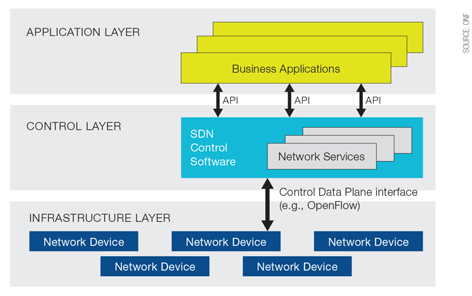
\includegraphics[scale=0.6]{fotos/2_MarcoTeorico/sdn_filosofia.png}
 \caption{Filosofia SDN.}
 \label{filosofiasdn}
\end{figure}

Como se puede observar, la interconexión entre las capas, se da gracias a las “interfaces” que se clasifican en “Southbound Interfaces” y en “Northbound Interfaces” haciendo referencia a la capa de abajo y arriba respectivamente.

\vspace{0.5cm}

Particularmente, la interfaz “norte” son interfaces de programación (API) - generalmente de alto nivel - que permiten la conexión con elementos externos con diferentes objetivos. Por ejemplo, una API puede ser desarrollada para que la información de la red se muestre en una página web.

\vspace{0.5cm}

Finalmente, la interfaz “sur” se trata de la comunicación entre los activos de la red y el controlador. En esta comunicación se hacen especialmente importantes protocolos como Openflow, ya que vinculan comunicaciones provenientes de elementos de la red con el controlador y sin ellos, no se podría generar la separación fundamental de SDN.

\vspace{0.5cm}

La filosofía detrás de SDN, similar a la del software Open Source, es decir que busca lograr la desvinculación de hardware y protocolos propietarios junto con la aceptación de estándares abiertos (como Openflow) que permitan la “liberación” o “universalidad” de la programación independientemente de marcas o compañías que lideran los avances con software propietario. 



\section{Openflow}
\label{marco_openflow}

Openflow es el protocolo abierto de comunicación utilizado entre el controlador SDN y los switches de la topología. Su especificación está dada por la Open Networking Foundation (ONF) que es el ente, sin fines de lucro, encargado de liderar la transformación de la infraestructura de las redes actuales, de acuerdo a su Misión.

\vspace{0.5cm}

Éste protocolo, es lo que permite la separación de los planos de Control y de Datos descritos en la idea fundamental de SDN. Gracias a él, es posible implementar la inteligencia (Control) en un bloque dedicado a este tipo de procesamiento. Liberando de responsabilidades al equipamiento encargado del switcheo y enrutamiento.

\vspace{0.5cm}

Los switches que implementan Openflow, contarán con la siguiente estructura lógica en su interior:

\begin{figure}[ht]
 \centering
 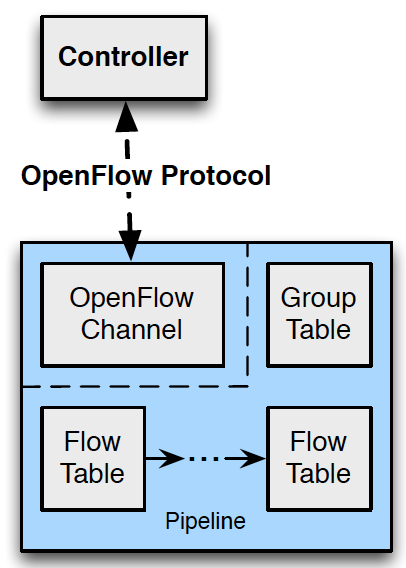
\includegraphics[scale=0.5]{fotos/2_MarcoTeorico/openflow_diagram.png}
 \caption{Diagrama Openflow.}
 \label{openflowdiagram}
\end{figure}


El funcionamiento de estos switches, vendrá dado por una lógica de “Tablas de flujo” o “Flow Tables”. Cada Tabla de Flujo está compuesta por “entradas de flujo” o “flow entries” que pueden ser agregadas, modificadas o eliminadas según se programe. En cada entrada, se definirán acciones sencillas para ejecutar, por ejemplo, reenvío (o “forwarding”), encapsulamiento o descarte del paquete.

\vspace{0.5cm}

Un paquete puede ser procesado por una tabla de flujo y luego ser enviado a otra tabla del Pipeline para continuar su tratamiento. Esto trae flexibilidad y permite tener gran granularidad a la hora de desarrollar y crear Tablas de Flujo con funciones específicas.

\vspace{0.5cm}

La tablas de flujo en Openflow, tienen una estructura dada compuesta por los siguientes campos:

\vspace{0.5cm}

Match Field: es el criterio de coincidencia que se utilizará para ejecutar la acción. Es el puerto de ingreso del paquete junto con información de la cabecera que está disponible y puede ser manipulada.

\vspace{0.5cm}

Prioridad: para dar un orden de ejecución y es definido por el programador según entienda necesario.

\vspace{0.5cm}

Contadores: para llevar actualizada la cantidad de veces que hubo un “match” con la entrada.

\vspace{0.5cm}

Instrucciones: conjunto de acciones a ejecutar. 

\vspace{0.5cm}

Timeouts: las entradas tienen un tiempo de vida útil acotado por estos timeouts

\vspace{0.5cm}

“Soft timeout”: la entrada se elimina si no hay “match” durante un tiempo mayor al “soft timeout”.

\vspace{0.5cm}

“Hard timeout”: si no es ‘0’, la entrada se elimina luego de existir por un tiempo superior al “hard timeout” sin importar si hubo “match”.

\vspace{0.5cm}

Cookies: puede usarse a modo opcional como valor extra para entradas que dependan de cierta estadística. No se utiliza cuando se procesan paquetes.

\vspace{0.5cm}
	
Finalmente, se debe aclarar que toda Tabla de Flujo cuenta con una entrada llamada “Table Miss Entry” de prioridad 0, que se utiliza cuando no hubo coincidencia para ninguna de las entradas anteriores. Puede generar que se envíe el paquete al Controlador, que lo descarte o que lo envíe a otra Tabla de Flujo.

\vspace{0.5cm}

Además de las ya definidas “Flow Entries” el switch Openflow estará compuesto por una Tabla de Grupo o “Group Table” y análogamente, las Tablas de Grupo están formadas por Entradas de Grupo o “Group Entries” que se diferencian en su identificador de grupo o “Group Identifier”.

\vspace{0.5cm}

A su vez, similar a las Tablas de Flujo, las Tablas de Grupo se tienen una estructura dada por los siguientes campos:

\vspace{0.5cm}

Identificador de grupo: es un entero único para diferenciar un grupo de los demás.

\vspace{0.5cm}

Tipo de grupo: se utiliza para representar el comportamiento del grupo. Los switches deben soportar los tipos “indirect” y “all” mientras que opcionalmente pueden soportar a su vez “select” y “fast failover”.

\vspace{0.5cm}

Indirect: grupos que soportan un solo “action bucket”. Permiten varias entradas de flujo y entradas de grupo en un mismo identificador de grupo lo que los convierte en grupos de convergencia rápida y  eficiente. Son los más simples, por lo que es normal que los switches soporten una gran cantidad de ellos en relación a los demás tipos.

\vspace{0.5cm}

All: grupos que ejecutan todos los “buckets” del mismo. Son usados en Multicast y Broadcast dado que permiten clonar efectivamente el paquete en diferentes “buckets”.

\vspace{0.5cm}

Select: grupos que soportan un solo “action bucket”. Los paquetes son procesados por el “bucket” seleccionado de acuerdo a un algoritmo externo a Openflow.

\vspace{0.5cm}

Fast Failover: grupos que ejecutan el primer “action bucket” vivo. Cada “bucket” está asociado a un puerto o grupo que maneja su estado de “vida”. Estos grupos deben implementar un mecanismo para detectar estos cambios de estado.

\vspace{0.5cm}

Contadores: contador que se actualiza cada vez que un paquete es procesado en el grupo.

\vspace{0.5cm}

“Action Buckets”: es el conjunto de acciones a ejecutar sobre un paquete.

\subsection{Openflow 1.3}
\label{openflow13}

OpenFlow 1.3

\section{Multicast}
\label{marco_multicast}

Los métodos de comunicación dentro de una red se pueden clasificar en tres categorías dependiendo en la cantidad de los receptores:
Uno de ellos, es  la comunicación unicast - relación uno a uno - que involucra a un único remitente y receptor. 

\vspace{0.5cm}

Luego se encuentra el método broadcast - relación uno a todos - que consiste en enviar paquetes a todos los integrantes de la red 
Y por último se encuentra el  método Multicast - relación uno a varios - que puede tener variaciones en la cantidad de remitentes, puede ser de uno a muchos o de muchos a muchos.

\vspace{0.5cm}

En la siguiente imagen se muestran las diferencias entre cada método de comunicación.

foto

\vspace{0.5cm}

Una forma de realizar Multicast es utilizar múltiples conexiones unicast para enviar la misma información a los destinatarios pero no se utiliza de forma eficiente la red y tampoco es escalable debido a que aumenta la carga de trabajo en los emisores y se consume más ancho de banda de la red. Para evitar estos problemas la red realiza copias adicionales a partir de la información original para asegurar que a cada destino le llegue una, generando una menor carga de trabajo y procesamiento en los elementos que conforman la red reduciendo el costo de recursos de esta. Por último provoca que la red sea menos propensa a “embotellamientos”, y por lo tanto que se encuentre más disponible para su uso. 

\vspace{0.5cm}

Respecto de los envíos de unicast y broadcast, las técnicas de Multicast presentan ventajas para transmitir la misma información a un grupo de receptores generando el uso más eficiente e inteligente del ancho de banda requerido al utilizar sólo una dirección Multicast para el grupo. 

\vspace{0.5cm}

Como en broadcast, Multicast tiene designado un rango de direcciones. Las cuales se encuentran en el rango 224.0.0.0/4, que pueden ser utlizadas para ruteo y en Internet. Presentan como ventaja que la tarjeta de red sólo va a aceptar la información dirigida a una dirección Multicast si la ha solicitado, al contrario de broadcast donde se realiza una inundación en la red.

\vspace{0.5cm}

Multicast se encuentra basado en el concepto de grupos, formados por los destinatarios que soliciten contenido de determinada dirección Multicast, la cual se puede enviar de forma eficiente en una sola transmisión. Cada integrante de un grupo puede enviar y recibir contenido de la dirección Multicast sin importar su ubicación geográfica, puede estar ubicado en cualquier lugar de Internet o en una red privada.

\vspace{0.5cm}

Para unirse o dejar de pertenecer a un grupo Multicast se utiliza el protocolo Internet Group Management Protocol (IGMP). 

\vspace{0.5cm}

IGMP es un protocolo utilizado por sistemas IPV4 para reportar la unión de un host a un grupo Multicast, también para informar la salida de del host del grupo y para obtener el estado de los grupos Multicast formados en la red.

\vspace{0.5cm}

Las funciones de IGMP realizan dos acciones. Cuando un receptor se une a un grupo Multicast, envía un mensaje IGMP para unirse al grupo (Membership Report) con la dirección IP Multicast del grupo al que quiere unirse.

\vspace{0.5cm}

La otra acción está relacionada con la pertenencia dinámica a los grupos. Para esto se designa un switch o un router de la red que sondea de forma periódica mediante un mensaje IGMP de solicitud de pertenencia a grupos (Host Membership Query Message) a los vecinos de la red. De esta forma se determina si se mantienen como miembros activos de grupos. Este mensaje es enviado a la dirección reservada 224.0.0.1, el cual tiene definido un Time to Leave (TTL) de valor uno. Si no se obtiene respuesta al mensaje de pertenencia por parte de un host, se deja de enviarle información y no se anuncia su dirección a las fuentes de datos del grupo al cual pertenecía. 

\vspace{0.5cm}

Hay tres versiones implementadas del protocolo, IGMPv1, IGMPv2 e IGMPv3, las cuales son explicadas en la siguiente sección (IGMP).

\vspace{0.5cm}

Con el protocolo IGMP se obtiene el conocimiento de cómo se encuentran formados los grupos Multicast, en consecuencia se conocen las fuentes de información y los receptores interesados. Resta conocer las rutas que debe utilizar el tráfico Multicast de origen a destino. Esta labor puede ser llevada a cabo por varios protocolos de enrutamiento que se encargan de construir los árboles de tráfico Multicast. Los cuales emplean  uno de los dos métodos básicos dependiendo de la cantidad de miembros que tenga el grupo. En base a ello se encuentran:

\vspace{0.5cm}
Protocolos de Enrutamiento de Modo Denso

\vspace{0.5cm}
Protocolos de Enrutamiento de Modo Disperso

\vspace{0.5cm}

Árboles de distribución Multicast

\vspace{0.5cm}

Los árboles de distribución son formados a medida que los receptores se van uniendo o saliendo de los grupos Multicast. Son determinados por los caminos de enrutamiento del tráfico desde el origen a los receptores. 

\vspace{0.5cm}

Hay dos tipos de árboles:

\vspace{0.5cm}

Short Path Tree (SPT)

\vspace{0.5cm}

Rendezvous Point Tree


\vspace{0.5cm}

Short Path Tree

\vspace{0.5cm}

Los SPT también llamados Árboles Basados en Origen definen un árbol de distribución para cada origen de tráfico Multicast que lo conecta con los receptores. Este tipo de árboles son usados por protocolos de Multicast en modo denso como DVMRP, PIM-DM y MOSPF. Para enviar el tráfico emplean el camino más corto entre el origen y destino tomando en cuenta la métrica de acuerdo a los saltos o la métrica de velocidad, referida al camino de menor retraso. La siguiente figura muestra tres árboles SPT desde la fuente hasta tres receptores. Gracias a esto crea una ruta óptima entre el origen y los participantes, garantizando un tiempo mínimo de retardo.

foto

Rendezvous Point Tree	

\vspace{0.5cm}

En los RPT el camino del tráfico se encuentra arraigado al router designado como Rendezvouz Point (RP) y no a la fuente del tráfico. Este tipo de árboles son usados por el protocolo PIM-SM. Los routers de la red encaminan la información de varias fuentes al RP y el RP se encarga de redirigirla a los receptores. En el modelo RPT los routers no tienen que conocer donde se ubican las fuentes de cada grupo Multicast, sólo necesitan conocer dónde se encuentra el RP. El RP debe descubrir las fuentes de cada grupo Multicast. En la siguiente imagen se muestra un ejemplo de árbol RPT.

foto

\vspace{0.5cm}

Multicast Forwarding 

\vspace{0.5cm}

En una transmisión unicast el tráfico es enviado a través de la red por un solo camino, de origen a destino. En Multicast la fuente envía información a una dirección que representa un grupo Multicast, el router debe identificar qué dirección está en sentido ascendente (hacia la fuente) y cuál se encuentra en sentido descendente. El concepto de encaminar tráfico lejos de la fuente, o sea hacia al receptor, se denomina Reverse Path Forwarding (RPF) .

\vspace{0.5cm}

RPF permite a los routers encaminar tráfico Multicast hacia abajo por el árbol de distribución. Utiliza la tabla de ruteo unicast para determinar sus vecinos descendentes y ascendentes, de esta forma sólo va a encaminar un paquete si es recibido por la interfaz ascendente. Si el paquete es recibido por la interfaz descendente, termina siendo descartado. Gracias a este método de transmisión se evitan los loops en las redes que implementan Multicast.



\subsection{Multicast en Capa 2}
\label{mcast_l2}


\subsection{Multicast en Capa 3: IP Multicast}
\label{mcast_l3}
ip multicast


\section{Internet Group Management Protocol}

\subsection{IGMPv1}
\label{igmpv1}

Es la primera versión de IGMP y consta de sólo dos tipos de mensajes de control, Membership Report (MR), emitido por los hosts, y Membership Query (MQ), emitido por el router. No implementa un mecanismo para que un host abandone un grupo Multicast. Los receptores envían un MR y el router designado lo registra en el grupo. El router envía periódicamente un MQ para comprobar si al menos un receptor continúa interesado en recibir tráfico del grupo. 

\subsection{IGMPv2}
\label{igmpv2}

IGMPv2 implementa la misma funcionalidad básica de IGMPv1. Se diferencia en que introduce un nuevo tipo de mensaje para abandonar el grupo Multicast, llamado Leave Group (LG). Gracias a este mensaje se identifica inmediatamente los receptores que ya no desean pertenecer al grupo Multicast. Cuando un host quiere abandonar el grupo envía un mensaje LG a la dirección Multicast 224.0.0.2. El router envía un mensaje MQ al grupo que el host quiere abandonar, si el host no responde con un MR, entonces se le deja de enviar tráfico al host. Si no se recibe ningún MR de parte del grupo se elimina el grupo Multicast.

\vspace{0.5cm}

IGMPv2 especifica dos modalidades de consulta, General Query y Group Specific Query. General Query es la utilizada por IGMPv1 y Group Specific Query permite realizar la consulta a los integrantes de determinado grupo.


\subsection{IGMPv3}
\label{igmpv3}

IGMPv3 agrega con respecto a las versiones anteriores, la funcionalidad de permitir que un receptor solicite recibir o dejar de recibir tráfico de una fuente o varias determinadas pertenecientes a un grupo. También añade otro tipo de mensaje de consulta, Group and Source Specific Query, para preguntar qué receptor continúa interesado en recibir tráfico Multicast de varias fuentes o una fuente concreta.

\subsection{Protocolos de enrutamiento}

Los protocolos de enrutamiento de Multicast IP siguen uno de los dos enfoques básicos determinados por la distribución de los miembros del grupo Multicast en toda la red.

\vspace{0.5cm}

El primer enfoque se basa en suponer que los miembros del grupo Multicast se distribuyen densamente en la red, es decir, muchas de las subredes contienen al menos un receptor del grupo. Esto se denomina Enrutamiento de Modo Denso y se basa en una técnica llamada inundación (se le envía el tráfico a todos los integrantes de la red) para propagar la información de todas las fuentes de tráfico Multicast de la red.

\vspace{0.5cm}

El segundo enfoque se basa en que los miembros del grupo se encuentran muy dispersos en la red y el ancho de banda disponible no es abundante. Esto ocurre en muchas regiones de Internet. En este caso inundar la red causaría un uso innecesario del ancho de banda disponible provocando el saturamiento de la red. Por lo tanto este modo debe emplear técnicas más selectivas para configurar los árboles de Multicast y se le llama 

\vspace{0.5cm}

Enrutamiento de Modo Disperso.

\vspace{0.5cm}

Protocolos de Enrutamiento de Modo Denso

\vspace{0.5cm}	

Entre los protocolos de enrutamiento de este modo existen los siguientes:

\vspace{0.5cm}

Distance Vector Multicast Protocol (DVMRP)

\vspace{0.5cm}

Multicast Open Shortest Path First (MOSPF)

\vspace{0.5cm}

Protocol Independent Multicast Dense Mode (PIM-DM)

\vspace{0.5cm}

Protocolos de Enrutamiento de Modo Disperso

\vspace{0.5cm}

Los protocolos de Enrutamiento de Modo Disperso es utilizado para grupos de receptores dispersos y alejados, no realizan una inundación como los de modo denso sino que envían tráfico sólo a los receptores interesados. Debido a esto son implementados en entornos donde se tiene disponible un ancho de banda acotado. Un protocolo de enrutamiento de este modo es el siguiente:
Protocol Independent Sparse Mode (PIM-SM)


\section{Protocol Independent Multicast (PIM)}
\label{marco_pim}
PIM es un protocolo desarrollado con el objetivo de estandarizar el enrutamiento Multicast que puede proporcionar un enrutamiento entre dominios a través de Internet, independientemente de los mecanismos proporcionados por los protocolos de enrutamiento unicast. Presenta dos modos operativos, uno para grupos Multicast densamente distribuidos (PIM-DM) y otro para grupos de distribución dispersa (PIM-SM).


\subsection{PIM Sparse Mode}
\label{pimsm}

En PIM-SM no se envía tráfico Multicast salvo que un receptor lo requiera. Para distribuir el tráfico se utilizan árboles RPT donde el RP se fija como punto de encuentro para los paquetes que se envían de las fuentes a los hosts. Entonces cada router si recibe tráfico Multicast lo va a enviar al RP y cada router que quiera recibir tráfico se va a dirigir al router RP.

\vspace{0.5cm}

A continuación se explica el funcionamiento del protocolo mediante un ejemplo. El ejemplo consiste en un servidor, que se encuentra realizando streaming a la dirección de Multicast 239.1.1.1 y el router R6 recibe un IGMP Membership Report desde un host conectado que desea recibir tráfico desde el servidor.

foto

El router R6 va a poder encontrar el servidor gracias al router RP, como fue mencionado anteriormente. El router R6 puede encontrar el RP de dos formas. Una es configurando manualmente la dirección del RP en cada router de la red, la otra es gracias a un protocolo que realiza la función de descubrir la red.  

\vspace{0.5cm}

Para recibir el tráfico Multicast el host debe enviar un mensaje IGMP Membership Report el router R6. Luego el router envía el mensaje hacia el RP para notificar del host interesado en el tráfico. En la siguiente imagen se muestra lo mencionado anteriormente.

foto

Cuando el RP recibe el mensaje IGMP comienza a enviar el tráfico hacia el host. El concepto de unirse al RP se le llama Rendezvous Path Tree (RPT). Cada grupo Multicast puede tener diferentes RP designados y también varias fuentes de tráfico. En la siguiente imagen se muestra el RPT formado.

foto

Por último PIM-SM tiene la funcionalidad de calcular la ruta más corta desde la fuente del tráfico al receptor. Cambia de un Rendezvous Path Tree a un Short Path Tree. Cuando obtiene la ruta más corta envía mensajes de tipo prune para eliminar la ruta utilizada anteriormente. De esta forma no se va a utilizar más el RP para el tráfico hacia ese receptor desde esa fuente.

\vspace{0.5cm}

En la siguiente imagen se muestra el cambio realizado en la ruta.


\subsection{PIM Dense Mode}
\label{pimdm}

PIM-DM.

\vspace{0.5cm}

PIM-DM es un protocolo de enrutamiento de modo denso, que construye árboles de tipo SPT inundando de tráfico Multicast la red y luego utiliza  pruning para eliminar las ramas donde no se encuentren receptores. 

\vspace{0.5cm}

En la siguiente imagen se muestra la inundación generada en la red.

foto

Cada router que reciba el tráfico Multicast va realizar una inundación en la red, provocando problemas. Uno son los loops de ruteo Multicast. Para evitarlos, los routers que no solicitaron el tráfico Multicast envían mensajes de tipo prune a los upstream routers (routers de donde se recibe el tráfico Multicast). Los mensajes prune se envían cuando el router no tiene hosts conectados directamente interesados en el tráfico Multicast, cuando no hay downstreams (routers a los cuales se envía el tráfico Multicast) routers interesados en el tráfico Multicast y cuando se recibe tráfico en una interfaz que no funciona como RPF.

\vspace{0.5cm}

Luego de eliminar los caminos no deseados para el tráfico se termina obteniendo lo que se llama un Short Path Tree (SPT). En la siguiente imagen se representa como queda el recorrido del tráfico.


foto

\subsection{Modelos de comuicación}

Multicast se clasifica en dos formas según el modo en que se envía la información. Uno es el Any Source Multicast (ASM) y el otro Source Specific Multicast (SSM). 

\vspace{0.5cm}

En Any Source Multicast se pueden tener varios servidores que envían información en un mismo grupo, utilizando la forma de intercambio de datos muchos a muchos. Para soportar el modelo muchos a muchos la red debe ser responsable del descubrimiento de la fuente. Cuando un host requiera unirse a un grupo, la red tiene que determinar todas las fuentes del grupo y enviárselas al host.

\vspace{0.5cm}

Source Specific Multicast se utiliza el método de envío de uno a muchos y la red no es responsable de saber dónde se encuentra la fuente de datos, ahora los hosts son los encargados de realizar esa función. Los hosts cuando se unen a un grupo especifican la fuente de donde quieren recibir la información y el grupo Multicast.

\vspace{0.5cm}

ASM y SSM no son protocolos, son modelos de servicio. Diferentes protocolos son implementados para poder realizarlos. Por ejemplo para SSM se utilizan los protocolos PIM-SM e IGMPv3.


\section{Open vSwitch}
\label{marco_openvswitch}

Open vSwitch

\section{Mininet}
\label{marco_mininet}

El software Mininet, es un emulador gratuito de elementos de redes SDN que puede representar virtualmente switches, routers y hosts clientes que emulan el kernel de Linux. Funciona  ya sea en un sistema Linux así como máquina virtual con otro sistema operativo lo que lo hace muy flexible para ambientes de investigación, desarrollo y enseñanza.

\vspace{0.5cm}

Además, permite la rápida creación de topologías complejas, testeo de desarrollos particulares, simulación de redes y todo sobre una misma consola. Es un proyecto de la ONF y por lo tanto, soporta el protocolo Openflow. En la imagen a continuación, se representa la “virtualización” posible gracias a Mininet, de los elementos físico de una posible red que se quiera emular:

Aca iria una foto.

Mininet provee ventajas respecto a los recursos necesarios para correr, la velocidad de booteo y la versatilidad respecto a los sistemas sobre los que corre. Además, es gratuito y de código abierto y con una comunidad que ha generado material y cursos útiles en varios sitios de internet.

\vspace{0.5cm}

Entre las ventajas, se contempla que la emulación de hosts, se hacen sobre el mismo kernel y esto permite la utilización de herramientas de networking y de línea de comandos disponibles en Linux. Por ejemplo, se pueden correr Scripts desde línea de comandos, se pueden correr servicios HTTP de pruebas, capturar paquetes con “tcpdump”, utilizar la herramienta “iperf” para testear capacidades y generar conexiones simultáneas o “scapy” para la generación de paquetes customizados entre muchas otras herramientas.

\vspace{0.5cm}

Respecto a las desventajas de Mininet, se encuentra la limitante física que impone el CPU y el ancho de banda disponible en el servidor donde corra. No es un emulador utilizado en ambientes de producción, sino más bien en entornos de investigación y desarrollo a pequeña o mediana escala.

foto



\section{Controlador RYU}
\label{marco_ryu}

El presente Proyecto será desarrollado utilizando aplicaciones del controlador RYU. Su significado, del japonés, es “flujo”. Este controlador, provee componentes de software sobre los cuales se pueden construir aplicaciones complejas para implementaciones de SDN. 

\vspace{0.5cm}

Es un software abierto cuyo código está disponible para todo público y soporta protocolos como Openflow, Netconf, OF-Config, etc. Está implementado totalmente en Python. Se integra con una gran variedad de switches reales de diferentes marcas y es compatible con Openstack.

\vspace{0.5cm}

Como desventaja, se podría señalar la falta de una interfaz gráfica para su configuración, como tienen otros controladores de SDN, aunque sí tiene un entorno gráfico para la visualización de las topologías llamado “Ryu Topology Viewer”.

\vspace{0.5cm}

Finalmente, dentro de las funcionalidades implementadas que vienen embebidas con RYU, se pueden mencionar el controlador simple switch py que está implementado para varias versiones de Openflow y, básicamente, permite el conocimiento de los host conectados a cierto switch y el armado de una tabla de direcciones MAC.


\chapter{Diseño del sistema.}

Notar que se genera una página nueva al iniciar un capítulo.

pepito

\section{Funcionalidades del sistema.}
\label{funcionalidades}



\section{Arquitectura del sistema.}
\label{arquitectura}


\section{Topologías.}
\label{topologias}

\subsection{Topologías lineales.}
\label{topos_lineales}
\subsection{Topologías "árbol".}
\label{topos_arbol}

\subsection{Topologías con loops.}
\label{topos_loops}


\subsection{Topologías full mesh.}
\label{topos_full_mesh}


\section{Controllador SDN.}

\subsection{Funcionalidades del controllador.}

\subsection{Librerías RYU.}

\subsubsection{Librería igmp.py.}

\subsubsection{Desarrollo paralelo a igmplib.py.}

\section{Menú inicial.}


\chapter{Desarrollo del sistema.}

\section{Controllador.}

\section{Menu inicial.}

\section{Scripts auxiliares.}

\subsection{App crea json}
das

\subsection{Algoritmo Dijkstra}
dijkstra
\subsection{Leer topo json}
dasd
\subsection{Streaming y recepción de contenido.}

\subsection{Impresión de información Openflow.}

\chapter{Pruebas y resultados.}
\label{pruebasyresultados}

En esta sección se detallarán las pruebas realizadas sobre el sistema para determinar el cumplimiento con los objetivos.

\section{Topologías lineales.}

\subsection{Topología lineal de 2 switches.}

\begin{figure}[ht]
 \centering
 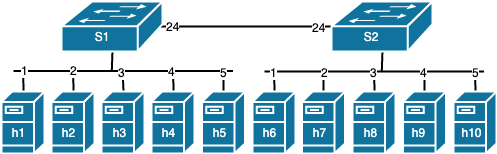
\includegraphics[width=1\textwidth]{fotos/5_Pruebas/1_topo_lineales/pequena.png}
 \caption{Topología lineal de 2 switches.}
 \label{topo_lineal_pequena}
\end{figure}


\vspace{0.5 cm}

\subsubsection{Caso de prueba 1: formación de un grupo Multicast.} 
Se utilizará \textit{iperf} para mostrar el procedimiento mediante el cual los \textit{hosts} se suscriben a un grupo Multicast. La IP del grupo será la 224.0.0.15 y se utilizará el host h1 para suscribirse al mismo.

\vspace{0.5cm}
Resultado esperado: se espera que el host envíe un \textit{Membership Report} hacia la IP del grupo y que el controlador cree el grupo con un identificador ya que reconoce que se trata un destino Multicast nuevo.


\vspace{0.5cm}
Resultado obtenido y explicación: 

Se observa en las figuras \ref{igmp_mr_h1} y \ref{igmp_mr_h1_detail} el paquete de \textit{Membership Report} proveniente del host 1 cuya IP es 10.0.0.11 y es enviada con destino la IP del grupo.

\begin{figure}[ht]
 \centering
 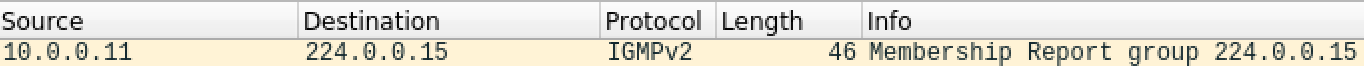
\includegraphics[width=1\textwidth]{fotos/5_Pruebas/1_topo_lineales/Casos/1/wire_igmp_de_host1.png}
 \caption{IGMP Membership report.}
 \label{igmp_mr_h1}
\end{figure}

\begin{figure}[ht]
 \centering
 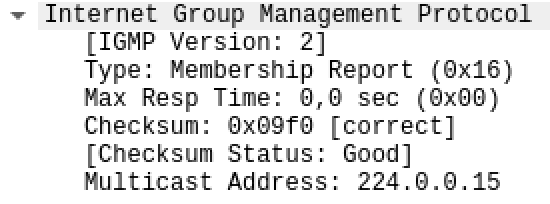
\includegraphics[width=0.6\textwidth]{fotos/5_Pruebas/1_topo_lineales/Casos/1/wire_igmp_detail.png}
 \caption{IGMP Membership Report - Detalle.}
 \label{igmp_mr_h1_detail}
\end{figure}



\vspace{0.5cm}
Mostrar recortes-capturas de tráfico con Wireshark mostrando paquetes importantes (Membership Report, Leave, etc).

\subsubsection{Caso de prueba 2: Streaming de video de 2 grupos Multicast} 
Se realiza streaming de video desde el Host X hacia la IP 225.0.0.20 (grupo A) y desde el Host Y hacia la IP 225.0.1.90 (Grupo B). El grupo A es recibido desde los host A, B, C y D. El grupo B es recibido desde los host E, F, G y H.

\vspace{0.5cm}
Resultado esperado: 

\vspace{0.5cm}
Resultado obtenido y explicación: 

\vspace{0.5cm}
Mostrar recortes-capturas de tráfico con Wireshark mostrando paquetes importantes (Membership Report, Leave, etc).

\subsubsection{Caso de prueba 3: Streaming de video de 5 grupos Multicast} 

Se realiza streaming.

\vspace{0.5cm}
Resultado esperado: 

\vspace{0.5cm}
Resultado obtenido y explicación: 

\vspace{0.5cm}
Mostrar recortes-capturas de tráfico con Wireshark mostrando paquetes importantes (Membership Report, Leave, etc).

\subsubsection{Caso de prueba 4: abandono de grupo Multicast} 

Se realiza streaming.

\vspace{0.5cm}
Resultado esperado: 

\vspace{0.5cm}
Resultado obtenido y explicación: 

\vspace{0.5cm}
Mostrar recortes-capturas de tráfico con Wireshark mostrando paquetes importantes (Membership Report, Leave, etc).

\subsubsection{Caso de prueba 5: eliminación de grupo Multicast} 
Se realiza streaming.

\vspace{0.5cm}
Resultado esperado: 

\vspace{0.5cm}
Resultado obtenido y explicación: 

\vspace{0.5cm}
Mostrar recortes-capturas de tráfico con Wireshark mostrando paquetes importantes (Membership Report, Leave, etc).

\subsubsection{Caso de prueba 5: efecto de la baja de un enlace.} 
Se realiza streaming.

\vspace{0.5cm}
Resultado esperado: 

\vspace{0.5cm}
Resultado obtenido y explicación: 

\vspace{0.5cm}
Mostrar recortes-capturas de tráfico con Wireshark mostrando paquetes importantes (Membership Report, Leave, etc).





\subsection{Topología lineal de 10 switches.}

\begin{figure}[ht]
 \centering
 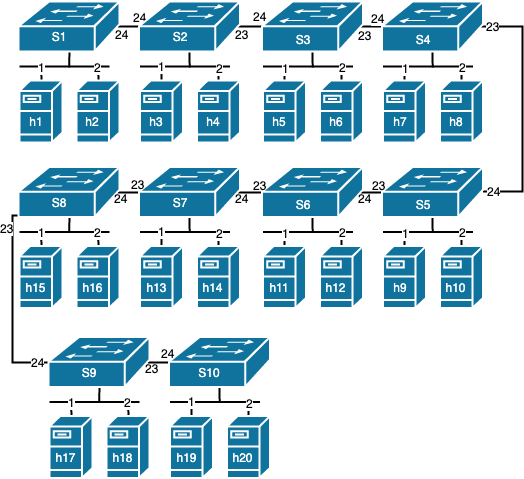
\includegraphics[width=0.9\textwidth]{fotos/5_Pruebas/1_topo_lineales/grande.png}
 \caption{Topología lineal de 10 switches.}
 \label{topo_lineal_grande}
\end{figure}


\subsubsection{Caso de prueba 1: Streaming de video de 5 grupos Multicast} 
Se realiza streaming.

\vspace{0.5cm}
Resultado esperado: 

\vspace{0.5cm}
Resultado obtenido y explicación: 

\vspace{0.5cm}
Mostrar recortes-capturas de tráfico con Wireshark mostrando paquetes importantes (Membership Report, Leave, etc).

\subsubsection{Caso de prueba 2: abandono de grupo Multicast} 

Se realiza streaming.

\vspace{0.5cm}
Resultado esperado: 

\vspace{0.5cm}
Resultado obtenido y explicación: 

\vspace{0.5cm}
Mostrar recortes-capturas de tráfico con Wireshark mostrando paquetes importantes (Membership Report, Leave, etc).

\subsubsection{Caso de prueba 3: eliminación de grupo Multicast} 
Se realiza streaming.

\vspace{0.5cm}
Resultado esperado: 

\vspace{0.5cm}
Resultado obtenido y explicación: 

\vspace{0.5cm}
Mostrar recortes-capturas de tráfico con Wireshark mostrando paquetes importantes (Membership Report, Leave, etc).

\subsubsection{Caso de prueba 5: efecto de la baja de un enlace.} 
Se realiza streaming.

\vspace{0.5cm}
Resultado esperado: 

\vspace{0.5cm}
Resultado obtenido y explicación: 

\vspace{0.5cm}
Mostrar recortes-capturas de tráfico con Wireshark mostrando paquetes importantes (Membership Report, Leave, etc).

\vspace{0.5cm}
NOTA: a partir de este punto, se asume que queda demostrado que el sistema cubre las necesidades básicas de gestión (alta, baja y modificación) de grupos Multicast.

\vspace{0.5cm}
Las siguientes pruebas en las demás topologías, serán para demostrar el efecto de la baja de enlaces en lo que respecta a la redirección del tráfico.


\section{Topologías de ``árbol''.}

\subsection{Topología de árbol con 3 ramificaciones.}

\begin{figure}[ht]
 \centering
 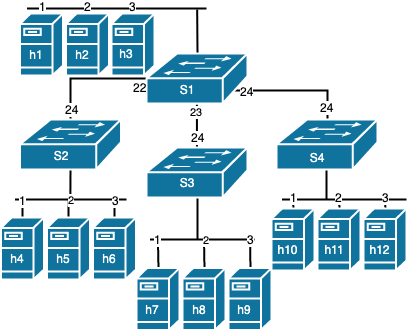
\includegraphics[width=0.9\textwidth]{fotos/5_Pruebas/2_topo_arbol/3ramas.png}
 \caption{Topología de arbol de 3 ramificaciones.}
 \label{topo_arbol_3_ramas}
\end{figure}

\subsubsection{Caso de prueba N:.} 
Se realiza streaming.

\vspace{0.5cm}
Resultado esperado: 

\vspace{0.5cm}
Resultado obtenido y explicación: 

\vspace{0.5cm}
Mostrar recortes-capturas de tráfico con Wireshark mostrando paquetes importantes (Membership Report, Leave, etc).




\subsection{Topología de árbol con 3 niveles de profundidad.}

\begin{figure}[ht]
 \centering
 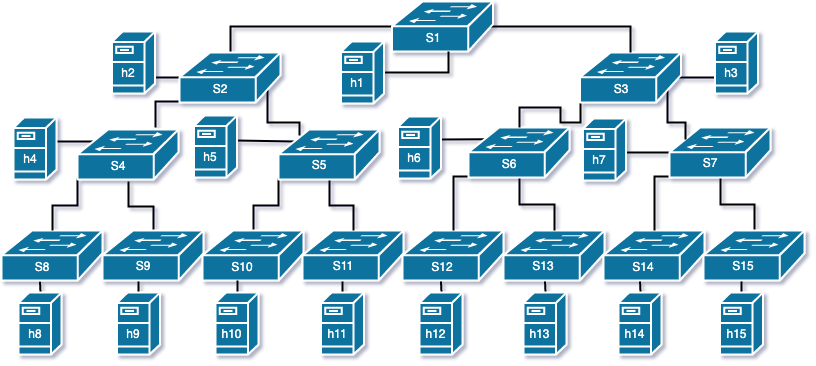
\includegraphics[width=0.9\textwidth]{fotos/5_Pruebas/2_topo_arbol/3niveles.png}
 \caption{Topología de arbol de 3 niveles de profundidad.}
 \label{topo_arbol_3_niveles}
\end{figure}

\subsubsection{Caso de prueba N:.} 
Se realiza streaming.

\vspace{0.5cm}
Resultado esperado: 

\vspace{0.5cm}
Resultado obtenido y explicación: 

\vspace{0.5cm}
Mostrar recortes-capturas de tráfico con Wireshark mostrando paquetes importantes (Membership Report, Leave, etc).

\section{Topologías de anillo.}

Intro.

\subsection{Anillo de 4 switches.}


\begin{figure}[ht]
 \centering
 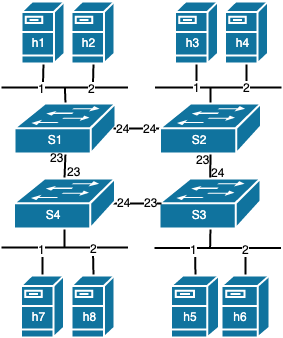
\includegraphics[width=0.5\textwidth]{fotos/5_Pruebas/3_topo_anillo/simple.png}
 \caption{Topología de anillo de 4 switches..}
 \label{anillo_simple}
\end{figure}

\subsubsection{Caso de prueba N:.} 
Se realiza streaming.

\vspace{0.5cm}
Resultado esperado: 

\vspace{0.5cm}
Resultado obtenido y explicación: 

\vspace{0.5cm}
Mostrar recortes-capturas de tráfico con Wireshark mostrando paquetes importantes (Membership Report, Leave, etc).

\subsection{Topología de árbol con anillos.}

\begin{figure}[ht]
 \centering
 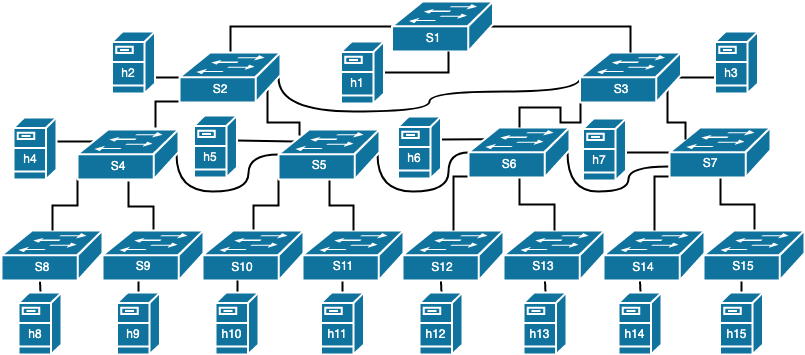
\includegraphics[width=0.7\textwidth]{fotos/5_Pruebas/3_topo_anillo/arbol_anillo.png}
 \caption{Topología de arbol con anillos.}
 \label{arbol_anillos}
\end{figure}

\subsubsection{Caso de prueba N:.} 
Se realiza streaming.

\vspace{0.5cm}
Resultado esperado: 

\vspace{0.5cm}
Resultado obtenido y explicación: 

\vspace{0.5cm}
Mostrar recortes-capturas de tráfico con Wireshark mostrando paquetes importantes (Membership Report, Leave, etc).


\section{Topologías full mesh.}

\subsection{Mesh de 4 switches.}

\begin{figure}[ht]
 \centering
 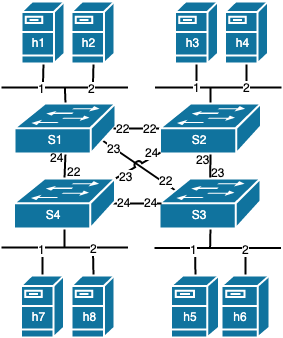
\includegraphics[width=0.5\textwidth]{fotos/5_Pruebas/4_topo_mesh/mesh_simple.png}
 \caption{Topología full mesh de 4 switches.}
 \label{mesh_simple}
\end{figure}

\subsubsection{Caso de prueba N:.} 
Se realiza streaming.

\vspace{0.5cm}
Resultado esperado: 

\vspace{0.5cm}
Resultado obtenido y explicación: 

\vspace{0.5cm}
Mostrar recortes-capturas de tráfico con Wireshark mostrando paquetes importantes (Membership Report, Leave, etc).

\subsection{Mesh de 6 switches.}

\begin{figure}[ht]
 \centering
 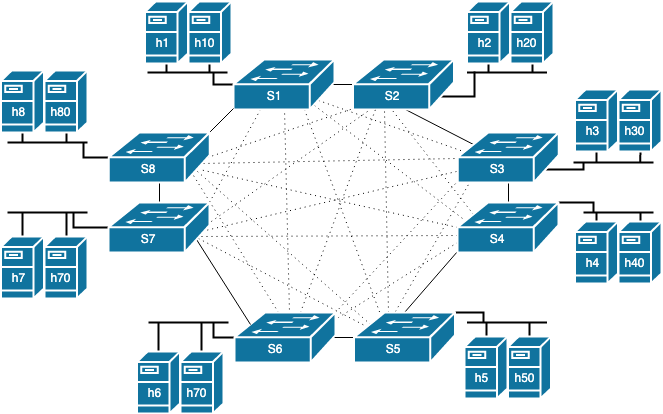
\includegraphics[width=0.7\textwidth]{fotos/5_Pruebas/4_topo_mesh/mesh_compleja.png}
 \caption{Topología full mesh de 6 switches.}
 \label{mesh_compleja}
\end{figure}

\subsubsection{Caso de prueba N:.} 
Se realiza streaming.

\vspace{0.5cm}
Resultado esperado: 

\vspace{0.5cm}
Resultado obtenido y explicación: 

\vspace{0.5cm}
Mostrar recortes-capturas de tráfico con Wireshark mostrando paquetes importantes (Membership Report, Leave, etc).


\chapter{Conclusiones}
\label{conclusiones}

Para incluir una referencia bibliográfica se utilizará el comando cite:~\cite{girard1989}.
Ejemplo de una cita múltiple:~\cite{ranta2012,tcs2015}.\\

También podemos utilizar el comando ref hacer referencia a una capítulo o sección que haya sido indexada con el comando label. Por ejemplo, la introducción, que es el Capítulo~\ref{intro}, o esta misma sección que es la~\ref{marcoteorico}. Ref también sirve para hacer referencia a  figuras, como la Figura~\ref{filosofiasdn}, que está más adelante en el texto.

LATEX.

Para incluir una referencia bibliográfica se utilizará el comando cite:~\cite{girard1989}.
Ejemplo de una cita múltiple:~\cite{ranta2012,tcs2015}.\\

También podemos utilizar el comando ref hacer referencia a una capítulo o sección que haya sido indexada con el comando label. Por ejemplo, la introducción, que es el Capítulo~\ref{pruebasyresultados}, o esta misma sección que es la~\ref{marcoteorico}. Ref también sirve para hacer referencia a figuras, como la Figura~\ref{anillo_simple}, que está más adelante en el texto.



\bibliographystyle{IEEEtran}
%%bibliography
%% No borrar estas dos líneas. Revisar de tener los archivos IEEETran y biblio.bib en la misma carpeta
%% si no están y no anda, correr el compilador de latex varias veces. Primero el bibtex, luego pdflatex, luego pdflatex otra vez.
\renewcommand{\bibname}{Referencias bibliográficas} 

\bibliography{biblio}

Datos bibliográficos mínimos según tipo de publicación:

\textbf{Libros:} autor(es), título del libro, edición (si no es la primera), editorial, ciudad de la editorial, año de publicación.

\textbf{Artículos de revista}: autor(es), título del articulo, nombre de la revista, volumen, numero, pagina inicial, pagina final, mes, año.

\textbf{Artículos de canales de conferencia:} autor(es), titulo del articulo, nombre d se la conferencia, ciudad de la conferencia, año.

\textbf{Pagina web:} Autor(es), titulo de la pagina, URL, fecha de accedido

\textbf{Tesis de grado/maestría/doctorado:} autor, título, tipo de tesis, departamento, universidad, ciudad de la universidad, año.


\appendix %A partir de acá los capítulos se enumerarán A, B, C, etc

\chapter{Herramientas utilizadas}

\section{Apache JMeter}
\label{AnexoJMeter}

Apache JMeter es una herramienta de software libre diseñada para realizar pruebas de carga y medidas de desempeño. Fue diseñada originalmente para testeo de aplicaciones Web pero con el paso del tiempo a ido evolucionando adicionando funciones de testeo.

\vspace{0.5cm}

Durante este proyecto se utiliza como generador de tráfico para conocer los limites del sistema bajo pruebas de alto tráfico. A continuación se detallará la configuración utilizada.

\vspace{0.5cm}

Primero se crea el \textit{Thread Group}. En él, se definen la cantidad de usuarios que consumirán (\textit{Number of Threads}), el tiempo en el que lo harán (\textit{Ramp-up Period}) y la cantidad de veces que se repitirá la acción(\textit{Loop Count}). Se puede observar un ejemplo en la figura.

\vspace{0.5cm}

% \begin{figure}[H]
%     \centering
%     \includegraphics[width=1\textwidth]{fotos/ThreadGroup.png}
%     \caption{Configuración JMeter - Thread Group}
%     \label{fig:JMeter_ThreadGroup}
% \end{figure}

\vspace{0.5cm}

Luego de ello, se deben configurar los datos del servidor, esto se realiza en la opción \textit{HTTP Request}. En esta opción, se agrega protocolo a utilizar, la IP y puerto del servidor, el método que usarán los pedidos y el \textit{PATH} desde donde se solicitará la información. La figura  muestra un ejemplo de configuración utilizado para realizar GET sobre un video.

\vspace{0.5cm}

Después de esto se ejecuta con la función \textit{Play} y se espera a que se detenga para obtener los resultados.

\vspace{0.5cm}

% \begin{figure}[H]
%     \centering
%     \includegraphics[width=1\textwidth]{fotos/HTTP_Request.png}
%     \caption{Configuración JMeter - HTTP Request}
%     \label{fig:JMeter_HTTPrequest}
% \end{figure}


\section{Network File System}
\label{seccA.2}

Network File System (NFS) es un protocolo diseñado para compartir archivos o carpetas entre sistemas con distribuciones Linux/Unix. En este proyecto se utiliza para montar archivos desde una VM para poder modificarlos desde otra VM que se encuentre en la misma red.

\vspace{0.5cm}

Usa la arquitectura estándar de servidor/cliente para compartir los archivos y carpetas. Para poder montarlo y compartir el archivo ``expires.conf'' del Origin Server se utiliza como referencia \cite{tecmint_NFS}.

\vspace{0.5cm}

Se tendrá, por lo tanto, que el servidor será el Origin Server y el cliente será el Backend.
En primera instancia se deben instalar los paquetes de NFS para luego iniciar el servicio. Se ejecutan los siguientes comandos (esto se realiza en ambas VM):

\vspace{0.5cm}

\begin{origin}
yum install nfs-utils nfs-utils-lib
/etc/init.d/portmap start
/etc/init.d/nfs start
chkconfig --level 35 portmap on
chkconfig --level 35 nfs on
\end{origin}

\vspace{0.5cm}

En el servidor, se debe especificar la locación a exportar. Esto se hace dentro del archivo ``/etc/exports'' de la siguiente forma:

% \begin{figure}[H]
%     \centering
%     \includegraphics[width=0.8\textwidth]{fotos/NFS_export.png}
%     \caption{Configuración NFS - Servidor}
%     \label{fig:NFS_export}
% \end{figure}

En este caso se comparte la carpeta ``/etc/httpd/conf.d'' que es donde se encuentra el archivo ``expires.conf''. Además, se le otorgan privilegios de leer y escribir al Backend.

\vspace{0.5cm}

Del lado del cliente se debe montar el directorio compartido por el servidor. Para esto se ejecuta primero el siguiente comando:

\vspace{0.5cm}

\begin{backend}
mount -t nfs origin.vcdn:/etc/httpd/conf.d /home/centos/cacheManual/expiresFile
\end{backend}

\vspace{0.5cm}

De esta forma queda montado el directorio ``/etc/httpd/conf.d'' en la carpeta ``/home/centos/cacheManual/expiresFile''. 

\vspace{0.5cm}

% Esta solución es temporal, para realizarlo de manera permanente se debe modificar el archivo ``/etc/fstab'' dentro del cliente. El procedimiento realizado tiene como resultado la configuración de la figura \ref{fig:NFS_fstab}.

% \begin{figure}[H]
%     \centering
%     \includegraphics[width=1\textwidth]{fotos/NFS_fstab.png}
%     \caption{Configuración NFS - Cliente}
%     \label{fig:NFS_fstab}
% \end{figure}


\section{Instalación de entorno de trabajo Django}
\label{seccA.3}

El entorno virtual \textit{virtualenv} es una herramienta utilizada para crear entornos aislados para Python, la cual permite gestionar programas, paquetes y mantener el entorno de desarrollo ordenado.  Luego de crearlo es necesario activarlo para poder utilizarlo.
A continuación se muestran los comandos para su creación y activación.

\vspace{0.5cm}
\begin{frontend}
 python3.6 -m venv env
 source env/bin/activate
\end{frontend}
\vspace{0.5cm}

Una vez instalado y activado el entorno virtual, es necesario instalar la librería propia de Django, en este caso se utilizó la versión 2.1.5.


\vspace{0.5cm}
\begin{frontend}
(env)pip install django
\end{frontend}
\vspace{0.5cm}

Recién en este momento el entorno de trabajo está listo para comenzar a desarrollar. 
El siguiente paso es iniciar el proyecto con el siguiente comando:


\vspace{0.5cm}
\begin{frontend}
django-admin startproject vCDN
\end{frontend}
\vspace{0.5cm}


Django trabaja con aplicaciones, con el siguiente comando se pueden crear las mismas. En este caso se optó por manejar tres aplicaciones distintas a las que llamamos: master, DNS y Files.

\vspace{0.5cm}
\begin{frontend}
python3.6 manage.py startapp portal
python3.6 manage.py startapp DNS
python3.6 manage.py startapp Files
\end{frontend}
\vspace{0.5cm}

El último paso es correr el servidor de desarrollo web propio de Django, el cual se activa con el siguiente comando.

\vspace{0.5cm}
\begin{frontend}
python3.6 manage.py runserver
\end{frontend}
\vspace{0.5cm}


\section{Instalación de DNS}
\label{seccA.4}
Para la instalación del DNS se generó un playbook que realiza todas las tareas necesarias. Se detalla a continuación el mismo mostrando una a una las tareas a completar.

\begin{lstlisting}[style=codigobase, caption= instalarDNS.yaml]
---
# Tareas para instalacion de Bind
- hosts: dns
  become: true
  tasks:
          - name: Instalar bind
            yum:
                    pkg: bind
                    state: installed
          - name: Copiar archivo named conf
            template:
                    src: ./named.conf.j2
                    dest: /etc/named.conf
                    owner: root
                    group: named
                    mode: 0660

          - name: Crear directorio named
            file:
                    path: /etc/named
                    state: directory
                    owner: root
                    group: named
                    mode: 0750

          - name: Copiar archivo named.local.conf
            template:
                    src: ./named.conf.local
                    dest: /etc/named/named.conf.local
                    owner: root
                    group: named
                    mode: 0660

          - name: Copiar archivo named.local.default
            template:
                    src: ./named.conf.default
                    dest: /etc/named/named.conf.default
                    owner: root
                    group: named
                    mode: 0660

          - name: Copiar archivo forward.vcdn.local para \
                  DNS interno
            template:
                    src: ./forward.vcdn.local
                    dest: /var/named/forward.vcdn.local
                    owner: root
                    group: named
                    mode: 0660

          - name: Copiar archivo reverse.vcdn.local para \
                  DNS interno
            template:
                    src: ./reverse.vcdn.local
                    dest: /var/named/reverse.vcdn.local
                    owner: root
                    group: named
                    mode: 0660
\end{lstlisting}


\chapter{Archivos de configuración}


\section{Archivo answers.cfg PackStack}
\label{seccB.1}
En este archivo se definieron todas los componentes y configuraciones que debía tener la instalación de PackStack. Los componentes a instalar son los mencionados durante este documento, para lo cual se debe asignar ``y'' o ``n''
en cada módulo.

\vspace{0.5cm}

Además se deben hacer configuraciones importantes en cuanto a la ubicación de esos componentes, los roles de cada servidor físico, y cómo se conectará el vDC con la red externa. Entre ellas se destacan:
\begin{itemize}
    \item \textbf{CONFIG\_CONTROLLER\_HOST} 
    
    IP del servidor de Control (línea 98)
    \item \textbf{CONFIG\_COMPUTE\_HOSTS} 
    
    IP de los servidores de Cómputo (línea 101)
    \item \textbf{CONFIG\_NETWORK\_HOSTS} 
    
    IP del servidor de Network (línea 106)
    \item \textbf{CONFIG\_AMQP\_HOST} 
    
    IP del servidor AMQP (línea 130)
    \item \textbf{CONFIG\_MARIADB\_HOST} 
    
    IP del servidor de base de datos de OpenStack (línea 154)
    \item \textbf{CONFIG\_NEUTRON\_OVS\_BRIDGE\_MAPPINGS} 
    
    Mapeo del bridge virtual para acceder a la red externa (línea 372)
    \item \textbf{CONFIG\_NEUTRON\_OVS\_BRIDGE\_IFACES} 
    
    Interfaz asociada al bridge virtual (línea 383)
    \item \textbf{CONFIG\_NEUTRON\_OVS\_EXTERNAL\_PHYSNET} 
    
    Nombre asignado a la red externa (línea 391)

\end{itemize}

\vspace{0.5cm}
\begin{lstlisting}[style=codigobase,  caption= answers.cfg]
[general]
# Path to a public key to install on servers. If a usable
# key has not been installed on the remote servers, the 
# user is prompted for a password and this key is install-
# ed so the password will not be required again.
CONFIG_SSH_KEY=/root/.ssh/id_rsa.pub

# Default password to be used everywhere (overridden by 
# passwords set for individual services or users).
CONFIG_DEFAULT_PASSWORD=Falta.Menos321

# The amount of service workers/threads to use for each 
# service. Useful to tweak when you have memory 
# constraints. Defaults to the amount of cores on the 
# system.
CONFIG_SERVICE_WORKERS=%{::processorcount}

# Specify 'y' to install MariaDB. ['y', 'n']
CONFIG_MARIADB_INSTALL=y

# Specify 'y' to install OpenStack Image Service (glance).
CONFIG_GLANCE_INSTALL=y

# Specify 'y' to install OpenStack Block Storage (cinder).
CONFIG_CINDER_INSTALL=y

# Specify 'y' to install OpenStack Shared File System 
# (manila).
CONFIG_MANILA_INSTALL=n

# Specify 'y' to install OpenStack Compute (nova).
CONFIG_NOVA_INSTALL=y

# Specify 'y' to install OpenStack Networking (neutron).
CONFIG_NEUTRON_INSTALL=y

# Specify 'y' to install OpenStack Dashboard (horizon).
CONFIG_HORIZON_INSTALL=y

# Specify 'y' to install OpenStack Object Storage (swift).
CONFIG_SWIFT_INSTALL=n

# Specify 'y' to install OpenStack Metering (ceilometer). 
# Note this will also automatically install gnocchi 
# service and configures it as the metrics backend.
CONFIG_CEILOMETER_INSTALL=y

# Specify 'y' to install OpenStack Telemetry Alarming 
# (Aodh). Note Aodh requires Ceilometer to be installed 
# as well.
CONFIG_AODH_INSTALL=y

# Specify 'y' to install OpenStack Events Service (panko).
CONFIG_PANKO_INSTALL=n

# Specify 'y' to install OpenStack Data Processing 
# (sahara). In case of sahara installation packstack 
# also installs heat.
CONFIG_SAHARA_INSTALL=n

# Specify 'y' to install OpenStack Orchestration (heat).
CONFIG_HEAT_INSTALL=y

# Specify 'y' to install OpenStack Container Infrastructur
# Management Service (magnum).
CONFIG_MAGNUM_INSTALL=n

# Specify 'y' to install OpenStack Database (trove)
CONFIG_TROVE_INSTALL=n

# Specify 'y' to install OpenStack Bare Metal Provisioning 
# (ironic).
CONFIG_IRONIC_INSTALL=n

# Specify 'y' to install the OpenStack Client packages 
# (command-line tools). An admin "rc" file will also be 
# installed.
CONFIG_CLIENT_INSTALL=y

# Comma-separated list of NTP servers. Leave plain if 
# Packstack should not install ntpd on instances.
CONFIG_NTP_SERVERS=

# Comma-separated list of servers to be excluded from the
# installation. This is helpful if you are running Pack-
# stack a second time with the same answer file and do not
# want Packstack to overwrite these server's configura-
# tions. Leave empty if you do not need to exclude any 
# servers.
EXCLUDE_SERVERS=

# Specify 'y' if you want to run OpenStack services
# in debug mode; otherwise, specify 'n'.
CONFIG_DEBUG_MODE=n

# Server on which to install OpenStack services specific 
# to the controller role (i.e, API servers or dashboard).
CONFIG_CONTROLLER_HOST=192.168.1.7

# List the servers on which to install the Compute service
CONFIG_COMPUTE_HOSTS=192.168.1.7,192.168.1.9

# List of servers on which to install the network service 
# such as Compute networking (nova network) or OpenStack 
# Networking (neutron).
CONFIG_NETWORK_HOSTS=192.168.1.7

# Specify 'y' if you want to use VMware vCenter as 
# hypervisor and storage; otherwise, specify 'n'.
CONFIG_VMWARE_BACKEND=n

# Specify 'y' if you want to use unsupported parameters.
# This should be used only if you know what you are doing.
# Issues caused by using unsupported options will not be 
# fixed before the next major release.
CONFIG_UNSUPPORTED=n

# Specify 'y' to enable the RDO testing repository.
CONFIG_ENABLE_RDO_TESTING=n

# Specify 'y' to enable RHEL optional repositories.
CONFIG_RH_OPTIONAL=y

# Service to be used as the AMQP broker. Allowed values
# are: rabbitmq ['rabbitmq']
CONFIG_AMQP_BACKEND=rabbitmq

# IP address of the server on which to install the 
# AMQP service.
CONFIG_AMQP_HOST=192.168.1.7

# Specify 'y' to enable SSL for the AMQP service.
CONFIG_AMQP_ENABLE_SSL=n

# Specify 'y' to enable authentication for the AMQP
# service.
CONFIG_AMQP_ENABLE_AUTH=n

# Password for the NSS certificate database of the 
# AMQP service.
CONFIG_AMQP_NSS_CERTDB_PW=PW_PLACEHOLDER

# User for AMQP authentication.
CONFIG_AMQP_AUTH_USER=amqp_user

# Password for AMQP authentication.
CONFIG_AMQP_AUTH_PASSWORD=PW_PLACEHOLDER

# IP address of the server on which to install MariaDB. If
# a MariaDB installation was not specified in 
# CONFIG_MARIADB_INSTALL, specify the IP address of an 
# existing database server (a MariaDB cluster can
# also be specified).
CONFIG_MARIADB_HOST=192.168.1.7

# User name for the MariaDB administrative user.
CONFIG_MARIADB_USER=root

# Password for the MariaDB administrative user.
CONFIG_MARIADB_PW=Falta.Menos321

# Password to use for the Identity service (keystone) to 
# access the database.
CONFIG_KEYSTONE_DB_PW=Falta.Menos321

# Enter y if cron job for removing soft deleted DB rows 
# should be created.
CONFIG_KEYSTONE_DB_PURGE_ENABLE=True

# Default region name to use when creating tenants in 
# the Identity service.
CONFIG_KEYSTONE_REGION=RegionOne

# Token to use for the Identity service API.
CONFIG_KEYSTONE_ADMIN_TOKEN=49ea2c75239c432eb2f15b99f854b9

# Email address for the Identity service 'admin' user.
CONFIG_KEYSTONE_ADMIN_EMAIL=root@localhost

# User name for the Identity service 'admin' user.
CONFIG_KEYSTONE_ADMIN_USERNAME=admin

# Password to use for the Identity service 'admin' user.
CONFIG_KEYSTONE_ADMIN_PW=Falta.Menos321

# Password to use for the Identity service 'demo' user.
CONFIG_KEYSTONE_DEMO_PW=Falta.Menos321

# Identity service API version string. ['v2.0', 'v3']
CONFIG_KEYSTONE_API_VERSION=v3

# Identity service token format (UUID, PKI or FERNET). The
# recommended format for new deployments is FERNET. 
CONFIG_KEYSTONE_TOKEN_FORMAT=FERNET

# Type of Identity service backend (sql or ldap).
CONFIG_KEYSTONE_IDENTITY_BACKEND=sql

# URL for the Identity service LDAP backend.
CONFIG_KEYSTONE_LDAP_URL=ldap://192.168.1.7

# Password to use for the Image service (glance) to access
# the database.
CONFIG_GLANCE_DB_PW=Falta.Menos321

# Password to use for the Image service to authenticate 
# with the Identity service.
CONFIG_GLANCE_KS_PW=Falta.Menos321

# Storage backend for the Image service (controls how the
# Image service stores disk images). Valid options are: 
# file or swift (Object Storage). The Object Storage ser-
# vice must be enabled to use it as a working backend; 
# otherwise, Packstack falls back to 'file'.
# ['file', 'swift']
CONFIG_GLANCE_BACKEND=file

# Password to use for the Block Storage service (cinder) 
# to access the database.
CONFIG_CINDER_DB_PW=Falta.Menos321

# Enter y if cron job for removing soft deleted DB rows 
# should be created.
CONFIG_CINDER_DB_PURGE_ENABLE=True

# Password to use for the Block Storage service to 
# authenticate with the Identity service.
CONFIG_CINDER_KS_PW=Falta.Menos321

# Storage backend to use for the Block Storage service;
# valid options are: lvm, gluster, nfs, vmdk, netapp, 
# solidfire.
CONFIG_CINDER_BACKEND=lvm

# Specify 'y' to create the Block Storage volumes group. 
# That is, Packstack creates a raw disk image in 
# /var/lib/cinder, and mounts it using a loopback device.
# This should only be used for testing on a proof-of-con-
# cept installation of the Block Storage service. A file-
# backed volume group is not suitable for production usage
CONFIG_CINDER_VOLUMES_CREATE=y

# Specify a custom name for the lvm cinder volume group
CONFIG_CINDER_VOLUME_NAME=cinder-volumes

# Size of Block Storage volumes group. Actual volume size 
# will be extended with 3% more space for VG metadata. 
# Remember that the size of the volume group will restrict
# the amount of disk space that you can expose to Compute 
# instances, and that the specified amount must be availa-
# ble on the device used for /var/lib/cinder.
CONFIG_CINDER_VOLUMES_SIZE=200G

# A single or comma-separated list of Red Hat Storage 
# (gluster) volume shares to mount. Example: 
# 'ip-address:/vol-name', 'domain:/vol-name'
CONFIG_CINDER_GLUSTER_MOUNTS=

# A single or comma-separated list of NFS exports to mount.
# Example: 'ip-address:/export-name'
CONFIG_CINDER_NFS_MOUNTS=

# Password to use for OpenStack Bare Metal Provisioning 
# (ironic) to access the database.
CONFIG_IRONIC_DB_PW=PW_PLACEHOLDER

# Password to use for OpenStack Bare Metal Provisioning to
# authenticate with the Identity service.
CONFIG_IRONIC_KS_PW=PW_PLACEHOLDER

# Enter y if cron job for removing soft deleted DB rows
# should be created.
CONFIG_NOVA_DB_PURGE_ENABLE=True

# Password to use for the Compute service (nova) to access
# the database.
CONFIG_NOVA_DB_PW=Falta.Menos321

# Password to use for the Compute service to authenticate 
# with the Identity service.
CONFIG_NOVA_KS_PW=Falta.Menos321

# Whether or not Packstack should manage a default initial
# set of Nova flavors. Defaults to 'y'.
CONFIG_NOVA_MANAGE_FLAVORS=y

# Overcommitment ratio for virtual to physical CPUs. 
# Specify 1.0 to disable CPU overcommitment.
CONFIG_NOVA_SCHED_CPU_ALLOC_RATIO=16.0

# Overcommitment ratio for virtual to physical RAM. 
# Specify 1.0 to disable RAM overcommitment.
CONFIG_NOVA_SCHED_RAM_ALLOC_RATIO=1.5

# Protocol used for instance migration. Valid options are:
# ssh and tcp. Note that the tcp protocol is not encrypted
# so it is insecure. ['ssh', 'tcp']
CONFIG_NOVA_COMPUTE_MIGRATE_PROTOCOL=ssh

# The hypervisor driver to use with Nova. Can be either
# 'qemu' or 'kvm'. Defaults to 'qemu' on virtual machines 
# and 'kvm' on bare metal hardware. For nested KVM set it 
# explicitly to 'kvm'.
CONFIG_NOVA_LIBVIRT_VIRT_TYPE=%{::default_hypervisor}

# Password to use for OpenStack Networking (neutron) to 
# authenticate with the Identity service.
CONFIG_NEUTRON_KS_PW=Falta.Menos321

# The password to use for OpenStack Networking to access
# the database.
CONFIG_NEUTRON_DB_PW=Falta.Menos321

# The name of the Open vSwitch bridge (or empty for 
# linuxbridge) for the OpenStack Networking L3 agent to 
# use for external  traffic. Specify 'provider' if you 
# intend to use a provider network to handle external 
# traffic.
CONFIG_NEUTRON_L3_EXT_BRIDGE=br-ex

# Password for the OpenStack Networking metadata agent.
CONFIG_NEUTRON_METADATA_PW=Falta.Menos321

# Specify 'y' to install OpenStack Networking's 
# Load-Balancing-as-a-Service (LBaaS).
CONFIG_LBAAS_INSTALL=y

# Specify 'y' to install OpenStack Networking's L3 
# Metering agent
CONFIG_NEUTRON_METERING_AGENT_INSTALL=y

# Specify 'y' to configure OpenStack Networking's
# Firewall-as-a-Service (FWaaS).
CONFIG_NEUTRON_FWAAS=n

# Specify 'y' to configure OpenStack Networking's 
# VPN-as-a-Service (VPNaaS).
CONFIG_NEUTRON_VPNAAS=n

# Comma-separated list of network-type driver entry points
# to be loaded from the neutron.ml2.type_drivers namespace
# ['local','flat', 'vlan', 'gre', 'vxlan', 'geneve']
CONFIG_NEUTRON_ML2_TYPE_DRIVERS=vxlan,flat

# Comma-separated, ordered list of network types to allo-
# cate as tenant networks. The 'local' value is only use-
# ful for single-box testing and provides no connectivity
# between hosts.['local','vlan', 'gre', 'vxlan', 'geneve']
CONFIG_NEUTRON_ML2_TENANT_NETWORK_TYPES=vxlan

# Comma-separated ordered list of networking mechanism 
# driver entry points to be loaded from the neutron.ml2
# .mechanism_drivers namespace. ['logger', 'test', 
# 'linuxbridge', 'openvswitch', 'hyperv', 'ncs', 'arista'
# ,'cisco_nexus', 'mlnx', 'l2population','sriovnicswitch']
CONFIG_NEUTRON_ML2_MECHANISM_DRIVERS=openvswitch

# Comma-separated list of <vni_min>:<vni_max> tuples 
# enumerating ranges of VXLAN VNI IDs that are available
# for tenant network allocation. Minimum value is 0 and 
# maximum value is 16777215.
CONFIG_NEUTRON_ML2_VNI_RANGES=10:100

# Name of the L2 agent to be used with OpenStack Network-
# ing. ['linuxbridge', 'openvswitch', 'ovn']
CONFIG_NEUTRON_L2_AGENT=openvswitch

# Comma-separated list of bridge mappings for the Open-
# Stack Networking Open vSwitch plugin. Each tuple in the
# list must be in the format <physical_network>:
# <ovs_bridge>. Example: physnet1:br-eth1,physnet2:br-eth2
CONFIG_NEUTRON_OVS_BRIDGE_MAPPINGS=extnet:br-ex

# Comma-separated list of colon-separated Open vSwitch
# <bridge>:<interface> pairs. The interface will be added 
# to the associated bridge. If you desire the bridge to be
# persistent a value must be added to this directive, also
# CONFIG_NEUTRON_OVS_BRIDGE_MAPPINGS must be set in order
# to create the proper port. This can be achieved from the
# command line by issuing the following command: packstack 
# -allinone --os-neutron-ovs-bridge-mappings=ext-net:br-ex  
# --os-neutron-ovs-bridge-interfaces=br-ex:eth0
CONFIG_NEUTRON_OVS_BRIDGE_IFACES=br-ex:enp0s25

# Name of physical network used for external network when
# enabling CONFIG_PROVISION_DEMO. Name must be one of the
# included in CONFIG_NEUTRON_OVS_BRIDGE_MAPPINGS. Example:
# --os-neutron-ovs-bridge-mappings="extnet:br-ex,physnet1:
# br-vlan" --os-neutron-ovs-bridge-interfaces="br-ex:eth1
# ,br-vlan:eth2" -os-neutron-ovs-external-physnet="extnet"
CONFIG_NEUTRON_OVS_EXTERNAL_PHYSNET=extnet

# Interface for the Open vSwitch tunnel. Packstack 
# overrides the IP address used for tunnels on this 
# hypervisor to the IP found on the specified interface 
# (for example, eth1).
CONFIG_NEUTRON_OVS_TUNNEL_IF=

# VXLAN UDP port.
CONFIG_NEUTRON_OVS_VXLAN_UDP_PORT=4789

# Comma-separated list of bridge mappings for the Open-
# Stack Networking Open Virtual Network plugin. Each 
# tuple in the list must be in the format <physical_net
# work>:<ovs_bridge>. Example: physnet1:br-eth1,
# physnet2:br-eth2,physnet3:br-eth3
CONFIG_NEUTRON_OVN_BRIDGE_MAPPINGS=extnet:br-ex

# Comma-separated list of Open vSwitch bridges that must 
# be created and connected to interfaces in compute nodes
# when flat or vlan type drivers are enabled. These bridge 
# must exist in CONFIG_NEUTRON_OVN_BRIDGE_MAPPINGS and
# CONFIG_NEUTRON_OVN_BRIDGE_IFACES. Example: --os-neutron
# -ovn-bridges-compute=br-vlan --os-neutron-ovn-bridge-
# mappings="extnet:br-ex,physnet1:br-vlan" --os-neutron-
# ovn-bridge-interfaces="br-ex:eth1,br-vlan:eth2"
CONFIG_NEUTRON_OVN_BRIDGES_COMPUTE=

# Name of physical network used for external network when
# enabling CONFIG_PROVISION_DEMO. Name must be one of the
# included in CONFIG_NEUTRON_OVN_BRIDGE_MAPPINGS. Example:
# --os-neutron-ovn-bridge-mappings="extnet:br-ex,physnet1
# :br-vlan" --os-neutron-ovn-bridge-interfaces="br-ex:eth1
# ,br-vlan:eth2" -os-neutron-ovn-external-physnet="extnet"
CONFIG_NEUTRON_OVN_EXTERNAL_PHYSNET=extnet

# Specify 'y' to set up Horizon communication over https.
CONFIG_HORIZON_SSL=n

# Password used by Orchestration service user to authenti-
# cate against the database.
CONFIG_HEAT_DB_PW=Falta.Menos321

# Encryption key to use for authentication in the Orches-
# tration database (16, 24, or 32 chars).
CONFIG_HEAT_AUTH_ENC_KEY=8afc705a22064093

# Password to use for the Orchestration service to authen-
# ticate with the Identity service.
CONFIG_HEAT_KS_PW=Falta.Menos321

# Specify 'y' to install the Orchestration CloudFormation 
# API.
CONFIG_HEAT_CFN_INSTALL=y

# Name of the Identity domain for Orchestration.
CONFIG_HEAT_DOMAIN=heat

# Name of the Identity domain administrative user for 
# Orchestration.
CONFIG_HEAT_DOMAIN_ADMIN=heat_admin

# Password for the Identity domain administrative user 
# for Orchestration.
CONFIG_HEAT_DOMAIN_PASSWORD=Falta.Menos321

# Specify 'y' to provision for demo usage and testing.
CONFIG_PROVISION_DEMO=n

# The name to be assigned to the demo image in Glance 
# (default "cirros").
CONFIG_PROVISION_IMAGE_NAME=cirros

# A URL or local file location for an image to download
# and provision in Glance (defaults to a URL for a recent
# "cirros" image).
CONFIG_PROVISION_IMAGE_URL=http://download.cirros-cloud.
                net/0.3.5/cirros-0.3.5-x86_64-disk.img

# Format for the demo image (default "qcow2").
CONFIG_PROVISION_IMAGE_FORMAT=qcow2

# User to use when connecting to instances booted 
# from the demo image.
CONFIG_PROVISION_IMAGE_SSH_USER=cirros

# Name of the uec image created in Glance used in 
# tempest tests (default "cirros-uec").
CONFIG_PROVISION_UEC_IMAGE_NAME=cirros-uec

# Specify 'y' to configure the Open vSwitch external 
# bridge for an all-in-one deployment (the L3 external 
# bridge acts as the gateway for virtual machines).
CONFIG_PROVISION_OVS_BRIDGE=y

# Password to use for Gnocchi to access the database.
CONFIG_GNOCCHI_DB_PW=Falta.Menos321

# Password to use for Gnocchi to authenticate with the 
# Identity service.
CONFIG_GNOCCHI_KS_PW=Falta.Menos321

# Secret key for signing Telemetry service (ceilometer)
# messages.
CONFIG_CEILOMETER_SECRET=3c0954bd0afe4b1b

# Password to use for Telemetry to authenticate with 
# the Identity service.
CONFIG_CEILOMETER_KS_PW=Falta.Menos321

# Ceilometer service name. ['httpd', 'ceilometer']
CONFIG_CEILOMETER_SERVICE_NAME=httpd

# Backend driver for Telemetry's group membership 
# coordination. ['redis', 'none']
CONFIG_CEILOMETER_COORDINATION_BACKEND=redis

# Whether to enable ceilometer middleware in swift proxy.
# By default this should be false.
CONFIG_ENABLE_CEILOMETER_MIDDLEWARE=n

# IP address of the server on which to install Redis
CONFIG_REDIS_HOST=192.168.1.7

# Port on which the Redis server listens.
CONFIG_REDIS_PORT=6379

# Password to use for Telemetry Alarming to authenticate 
# with the Identity service.
CONFIG_AODH_KS_PW=Falta.Menos321

# Password to use for Telemetry Alarming (AODH) to access
# the database.
CONFIG_AODH_DB_PW=Falta.Menos321
\end{lstlisting}


\section{Template Heat para definir Stack}
\label{seccB.2}

La creación de un Stack utiliza tres archivos de configuración (se especifica el template para crear un sabor Chico):

\begin{itemize}
    \item \textbf{template1.yaml} Donde se definen todos los componentes que tendrá el Stack, además de todas las configuraciones de escalación:
\end{itemize}   

\vspace{0,5cm}

\begin{lstlisting}[style=codigobase, caption= template.yaml]
description: Autoscale group, policy and alarm

parameters:
 subnet_id:
  type: string
  description: subnet privada
  default: private_subnet
 external_network_id:
  type: string
  description: UUID de la red externa
  default: 001fd561-8f42-4548-a42e-6a4ad3589197

resources:
 scaleup_group:
  type: OS::Heat::AutoScalingGroup
  properties:
   cooldown: 300
   desired_capacity: 2
   max_size: 5
   min_size: 1
   resource:
    type: OS::Nova::Server::Edge
    properties:
     pool: { get_resource: pool }
     metadata: {"metering.server_group": {get_param:
                                        "OS::stack_id"}}
     user_data_format: RAW
     user_data:
      str_replace:  
       template: |  
        #!/bin/bash
        /opt/ts/bin/trafficserver start

 scaleup_policy:
  type: OS::Heat::ScalingPolicy
  properties:
   adjustment_type: change_in_capacity
   auto_scaling_group_id: { get_resource: scaleup_group }
   cooldown: 300
   scaling_adjustment: 1

 scaledown_policy:
  type: OS::Heat::ScalingPolicy
  properties:
   adjustment_type: change_in_capacity
   auto_scaling_group_id: { get_resource: scaleup_group }
   cooldown: 300
   scaling_adjustment: -1

 cpu_alarm_high:
  type: OS::Aodh::GnocchiAggregationByResourcesAlarm
  properties:
   description: Scale up if CPU > 80%
   metric: cpu_util
   aggregation_method: mean
   granularity: 300
   evaluation_periods: 1
   threshold: 80
   resource_type: instance
   comparison_operator: gt
   alarm_actions:
    - str_replace:
       template: trust+url
       params:
      url: {get_attr: [scaleup_policy, signal_url]}
     query:
      str_replace:
       template: '{"=": {"server_group": "stack_id"}}'
      params:
       stack_id: {get_param: "OS::stack_id"}

 cpu_alarm_low:
  type: OS::Aodh::GnocchiAggregationByResourcesAlarm
  properties:
   description: Scale down if CPU < 20%  
   metric: cpu_util
   aggregation_method: mean
   granularity: 300
   evaluation_periods: 1
   threshold: 20
   resource_type: instance
   comparison_operator: lt
   alarm_actions:
    - str_replace:
       template: trust+url
       params:
        url: {get_attr: [scaledown_policy, signal_url]}
     query:
       str_replace:
        template: '{"=": {"server_group": "stack_id"}}'
        params:
         stack_id: {get_param: "OS::stack_id"}

 lb:
  type: OS::Neutron::LBaaS::LoadBalancer
  properties:
   vip_subnet: {get_param: subnet_id}
  
 listener:
  type: OS::Neutron::LBaaS::Listener
  properties:
   loadbalancer: {get_resource: lb}
   protocol: HTTP
   protocol_port: 80
  
 pool:
  type: OS::Neutron::LBaaS::Pool
  properties:
   listener: {get_resource: listener}
   lb_algorithm: ROUND_ROBIN
   protocol: HTTP
  
 lb_monitor: 
  type: OS::Neutron::LBaaS::HealthMonitor
  properties:
   pool: { get_resource: pool }
   type: HTTP
   http_method: GET
   url_path: /test
   expected_codes: 200 
   delay: 5
   max_retries: 5
   timeout: 5
       
 lb_floating:
  type: OS::Neutron::FloatingIP
  properties:
   floating_network_id: {get_param: external_network_id}
   port_id: {get_attr: [lb, vip_port_id]}
  
outputs:
 scaleup_policy_signal_url:
  value: {get_attr: [scaleup_policy, signal_url]}

 scaledown_policy_signal_url:
  value: {get_attr: [scaledown_policy, signal_url]}

\end{lstlisting}

\vspace{0,5cm}

\begin{itemize}
    \item \textbf{environment.yaml} Donde se define la ubicación del recurso de escalación personalizado OS::Nova:: Server::Edge
\end{itemize}   

\vspace{0,5cm}
\begin{lstlisting}[style=codigobase, caption= environment.yaml]
resource_registry:
 "OS::Nova::Server::Edge": /home/centos/lb_edge.yaml
\end{lstlisting}

\vspace{0,5cm}

\begin{itemize}
    \item \textbf{lb\_edge} Por último, las configuraciones que debe tener ese recurso personalizado, más específicamente las características de un Edge
\end{itemize}   

\vspace{0,5cm}
\begin{lstlisting}[style=codigobase,  caption= lb\_edge.yaml]
description: Template para definir la instancia Edge

parameters:
 metadata:
 type: json
 image:
  type: string
  default: EdgeImage
 flavor:
  type: string
  default: Normal
 key_name:
  type: string
  default: KeyPair
 network:
  type: string
  default: private
 subnet:
  type: string
  default: private_subnet
 external_network:
  type: string
  default: public
 availability_zone:
  type: string
  default: zona-2
  pool:
    type: string

resources:
 server:
 type: OS::Nova::Server
 properties:
  flavor: {get_param: flavor}
  image: {get_param: image}
  key_name: {get_param: key_name}
  metadata: {get_param: metadata}
  availability_zone: {get_param: availability_zone}
  user_data_format: {get_param: user_data_format}
  user_data: {get_param: user_data}
  networks:
   - port: { get_resource: port }

 port:
  type: OS::Neutron::Port
  properties:
   network: {get_param: network}
   security_groups:
    - default

 member:
  type: OS::Neutron::LBaaS::PoolMember
  properties:
   subnet: {get_param: subnet}
   pool: {get_param: pool}
   address: {get_attr: [server, first_address]}
   protocol_port: 8088
\end{lstlisting}

\vspace{0,5cm}


\chapter{Código implementado}

\section{Controlador v15}
\label{codigo_controlador}
Explicacion.

\vspace{0.5cm}

\begin{lstlisting}[style=codigobase,  label = cod_correrP, caption= controlador.py]

import sys
import os
from ryu.base import app_manager
from ryu.controller import ofp_event
from ryu.controller.handler import CONFIG_DISPATCHER, 
								MAIN_DISPATCHER, DEAD_DISPATCHER
from ryu.controller.handler import set_ev_cls
from ryu.ofproto import ofproto_v1_3
from ryu.lib.packet import packet
from ryu.lib.packet import ethernet
from ryu.lib.packet import ether_types
from ryu.lib.packet import ipv4
from ryu.lib.packet import igmp
from ryu.lib.packet import lldp
import json
import time
import datetime
import app_crea_json

from ryu.topology import event
from ryu.topology.api import get_all_switch, get_all_link, 
							get_switch, get_link
from ryu.lib import dpid as dpid_lib
from ryu.controller import dpset
import copy
from ryu.lib.dpid import dpid_to_str


PRIORITY_MAX = 2000
PRIORITY_MID = 900
PRIORITY_LOW = 800
PRIORITY_MIN = 700

TABLE_1 = 0
TABLE_2 = 10
TABLE_3 = 20


class Controlador(app_manager.RyuApp):
    OFP_VERSIONS = [ofproto_v1_3.OFP_VERSION]

    def __init__(self, *args, **kwargs):
        super(Controlador, self).__init__(*args, **kwargs)

        self.camino_grupos = {}

        self.topo_shape = TopoStructure()

        'Datos de control para el controlador'
        self.groupID = 0
        self.lista_grupos = {}
        self.switches_por_gid = {}
        self.datapath_switch = {}

        'Datos de la topologia en la cual el controlador funciona'
        self.conexion_switches = {}
        self.conexion_hosts_switches = {}
        self.caminos_completos = {}
        self.dpids = {}

        self.leer_json('salida_topo.json')


    '####EVENTOS####'

    @set_ev_cls(ofp_event.EventOFPSwitchFeatures, CONFIG_DISPATCHER)
    def switch_features_handler(self, ev):
        datapath = ev.msg.datapath
        ofproto = datapath.ofproto
        parser = datapath.ofproto_parser
        dpid = datapath.id

        self.obtener_datapath_switches(datapath)

        self.default_flows(datapath, parser, ofproto)

        self.topo_shape.switch_ports_state.setdefault(dpid, {})
        self.topo_shape.switch_ports_state[dpid].setdefault('puertos', {})
        self.obtener_puertos_switch(dpid)

    @set_ev_cls(ofp_event.EventOFPPacketIn, MAIN_DISPATCHER)
    def packet_in_handler(self, ev):
        "Handle incoming packets from a datapath"

        if ev.msg.msg_len < ev.msg.total_len:
            self.logger.debug("packet truncated: only %s of %s bytes",
                              ev.msg.msg_len, ev.msg.total_len)

        msg = ev.msg
        datapath = msg.datapath
        parser = datapath.ofproto_parser
        in_port = msg.match['in_port']

        # Parse the packet
        pkt = packet.Packet(msg.data)
        eth = pkt.get_protocols(ethernet.ethernet)[0]
        destino = eth.dst
        req_igmp = pkt.get_protocol(igmp.igmp)
        req_lldp = pkt.get_protocol(lldp.lldp)

        if not req_lldp:
            pktIPV4 = pkt.get_protocol(ipv4.ipv4)
            IPV4dst = pktIPV4.dst

        if req_igmp:

            if igmp.IGMP_TYPE_LEAVE == req_igmp.msgtype:
                'HAY QUE VER SI EL SWITCH ES DESTINO'
                'SI ES DESTINO TOMO IN PORT Y LO BORRO DE LA LISTA DE PUERTOS ASOCIADOS A ESE SWITCH DESTINO'
                'SI ES EL UNICO PUERTO ASOCIADO A ESE DESTINO BORRO EL DESTINO'
                if self.puerto_es_de_host(in_port, datapath)[0]:
                    self.manejo_leave(datapath, req_igmp.address, in_port)

            elif igmp.IGMP_TYPE_REPORT_V1 == req_igmp.msgtype or igmp.IGMP_TYPE_REPORT_V2 == req_igmp.msgtype:
                'HAY QUE VER SI EL IN PORT ES UN HOST Y SI PERTENECE A UN GRUPO'
                'SI EL GRUPO NO EXISTE SE CREA EL GRUPO'
                'SI EL GRUPO YA EXISTE SE MODIFICA EL GRUPO'
                if self.puerto_es_de_host(in_port, datapath)[0]:
                    self.manejo_report(datapath, IPV4dst, in_port)
            else:
                print('NO SE SOPORTA IGMPv3')

        else:
            if self.esMulticast(destino):

                if self.es_origen(datapath, in_port):

                    switch_origen = self.obtener_nombre_switch(datapath.id)

                    if IPV4dst in self.lista_grupos:

                        group_id = self.lista_grupos[IPV4dst]
                        self.camino_grupos[group_id]['origen'].update({switch_origen:in_port})
                        self.manejo_trafico_multicast(group_id, IPV4dst, switch_origen)

                    else:
                        print('NO EXISTE EL GRUPO {}'.format(IPV4dst))


    'Evento para reconocer cuando se agrega un switch con sus respectivos links a la topologia'
    @set_ev_cls(event.EventSwitchEnter)
    def handler_switch_enter(self, ev):
        self.topo_shape.topo_raw_switches = copy.copy(get_switch(self, None))
        self.topo_shape.topo_raw_links = copy.copy(get_link(self, None))
        for i,link in enumerate(self.topo_shape.topo_raw_links):
            self.topo_shape.links_info.setdefault(i, {})
            self.topo_shape.links_info[i].update({'switch_origen':link.src.dpid})
            self.topo_shape.links_info[i].update({'switch_destino':link.dst.dpid})
            self.topo_shape.links_info[i].update({'puerto_origen':link.src.port_no})
            self.topo_shape.links_info[i].update({'puerto_destino':link.dst.port_no})


    @set_ev_cls(ofp_event.EventOFPPortStatus, MAIN_DISPATCHER)
    def port_status_handler(self, ev):
        msg = ev.msg
        dp = msg.datapath
        ofp = dp.ofproto
        dpid_str = {'dpid': dpid_to_str(dp.id)}
        port = msg.desc
        reason = msg.reason
        dpid = dp.id

        if reason is dp.ofproto.OFPPR_ADD:
            self.logger.info('[port=%d] Port add.',
                             port.port_no, extra=dpid_str)

        elif reason is dp.ofproto.OFPPR_DELETE:
            self.logger.info('[port=%d] Port delete.',
                             port.port_no, extra=dpid_str)

        else:
            assert reason is dp.ofproto.OFPPR_MODIFY
            port_down = port.state & ofp.OFPPS_LINK_DOWN
            port_up = port.state & ofp.OFPPS_LIVE
            #print(port.state)
            if port_down and (self.topo_shape.switch_ports_state[dpid]['puertos'][port.port_no] == 'UP'):
                estado_puertos = []
                lista_links = []
                print('PUERTO {} DEL SWITCH {} DOWN'.format(port.port_no, dpid))
                #print(self.topo_shape.switch_ports_state)
                'CADA VEZ QUE SE CAE UN PUERTO HAY QUE VERIFICAR EN LOS LINKS DE LA TOPOLOGIA, SI LOS PUERTOS QUE UNEN'
                'DOS SWITCHES ESTAN DOWN, SE DA DE BAJA EL PUERTO QUE CONECTA AMBOS SWITCHES Y SE INFORMA QUE EL LINK'
                'ESTA CAIDO. LUEGO SE RECALCULAN CAMINOS'

                link = self.topo_shape.obtener_link_que_se_cayo(dpid, port.port_no)
                print(link)
                if link is not None:
                    if link not in self.topo_shape.links_down:
                        self.topo_shape.links_down.append(link)
                        #lista_links = self.topo_shape.recargar_links(link, port)
                        #self.topo_shape.topo_raw_links = copy.copy(lista_links)
                        #print(self.topo_shape.topo_raw_links)

                    print('EN LINK DOWN {}'.format(self.topo_shape.links_down))
                    self.topo_shape.switch_ports_state[dpid]['puertos'][port.port_no] = 'DOWN'
                    estado_puertos = self.topo_shape.ambos_puertos_link_down(link)
                    if estado_puertos[0] == True and estado_puertos[1] == True:
                        print('LINK DOWN QUE UNE EL SWITCH {} CON EL SWITCH {} EN LOS PUERTOS {} {}'.format(link.src.dpid, link.dst.dpid,
                                                                                                            link.src.port_no, link.dst.port_no))
                        self.eliminar_conexion_entre_switches(link.src.dpid, link.dst.dpid, link.src.port_no, link.dst.port_no)
                        self.recalcular_caminos()
                else:
                    print('NONETYPE EN DOWN {}'.format(self.topo_shape.links_down))
                    print('LINK ES NONETYPE')

            #if self.topo_shape.switch_ports_state.get(dpid) != None:
            if port_up and (self.topo_shape.switch_ports_state[dpid]['puertos'][port.port_no] == 'DOWN'):
                estado_puertos = []
                lista_links_aux = []
                lista_links = self.topo_shape.topo_raw_links

                'HAY QUE VER SI SE LEVANTAN AMBOS PUERTOS QUE CORRESPONDEN A UN LINK DE LA TOPOLOGIA Y SETEAR'
                'LOS PUERTOS CORRESPONDIENTES EN LA CONEXION ENTRE SWITCHES. LUEGO SE RECALCULAN CAMINOS'
                #print(self.topo_shape.switch_ports_state)
                print('PUERTO {} DEL SWITCH {} UP'.format(port.port_no, dpid))

                link = self.topo_shape.obtener_link_que_se_levanto(dpid, port.port_no)
                if link is not None:
                    # if link in self.topo_shape.links_down:
                        #lista_links_aux = self.topo_shape.agregar_link_up(link, port)
                        #lista_links.extend(lista_links_aux)
                        #lista_links = self.cargar_array(lista_links, lista_links_aux)
                        #self.topo_shape.topo_raw_links = copy.copy(lista_links)
                    print('EN LINK UP {}'.format(self.topo_shape.links_down))
                    self.topo_shape.switch_ports_state[dpid]['puertos'][port.port_no] = 'UP'
                    estado_puertos = self.topo_shape.ambos_puertos_link_down(link)
                    if estado_puertos[0] == False and estado_puertos[1] == False:
                        print('LINK UP QUE UNE EL SWITCH {} CON EL SWITCH {} EN LOS PUERTOS {} {}'.format(link.src.dpid, link.dst.dpid,
                                                                                                            link.src.port_no, link.dst.port_no))
                        self.agregar_conexion_entre_switches(link.src.dpid, link.dst.dpid, link.src.port_no, link.dst.port_no)
                        self.recalcular_caminos()
                        self.topo_shape.links_down.remove(link)

                else:
                    print('NONETYPE EN UP {}'.format(self.topo_shape.links_down))
                    print('LINK ES NONETYPE')


    '###########FUNCIONES###########'

    def cargar_array(lista_1, lista_2):
        for item in lista_2:
            lista_1.append(item)
        return lista_1

    def obtener_puertos_switch(self, dpid):
        switch = self.obtener_nombre_switch(dpid)
        for switch_aux in self.conexion_switches[switch]:
            #print(self.conexion_switches[switch][switch_aux])
            self.topo_shape.switch_ports_state[dpid]['puertos'].update({self.conexion_switches[switch][switch_aux]:'UP'})
        #print(self.topo_shape.switch_ports_state)


    def eliminar_conexion_entre_switches(self, dpid_1, dpid_2, puerto_1, puerto_2):
        lista_group_id = []
        buckets = []
        switch_1 = self.obtener_nombre_switch(dpid_1)
        switch_2 = self.obtener_nombre_switch(dpid_2)
        self.conexion_switches[switch_1].pop(switch_2)
        self.conexion_switches[switch_2].pop(switch_1)
        #self.borrar_puertos_switch_groupID(dpid_1, puerto_1, dpid_2, puerto_2)
        self.limpio_camino_grupos()
        self.limpio_switches_por_groupID()


    def agregar_conexion_entre_switches(self, dpid_1, dpid_2, puerto_1, puerto_2):
        lista_group_id = []
        switch_1 = self.obtener_nombre_switch(dpid_1)
        switch_2 = self.obtener_nombre_switch(dpid_2)
        print('switch 1 : {}'.format(switch_1))
        print('switch 2 : {}'.format(switch_2))
        self.conexion_switches[switch_1].update({switch_2:puerto_1})
        self.conexion_switches[switch_2].update({switch_1:puerto_2})
        #self.borrar_puertos_switch_groupID(dpid_1, puerto_1, dpid_2, puerto_2)
        self.limpio_camino_grupos()
        self.limpio_switches_por_groupID()


    def recalcular_caminos(self):
        diccionario_nuevo = {}
        diccionario_nuevo.update({'switches':self.conexion_switches})
        diccionario_nuevo.update({'dpids':self.dpids})
        diccionario_nuevo.update({'hosts':self.conexion_hosts_switches})
        filename = 'topo_nueva.json'
        with open(filename, 'w') as fd:
    	    fd.write(json.dumps(diccionario_nuevo))
        fd.close()
        os.system('python app_crea_json.py topo_nueva.json')
        self.leer_json('salida_topo.json')
        self.actualizo_camino_grupos()


    def actualizo_camino_grupos(self):

        for group_id in self.lista_grupos.values():
            IPV4dst = self.obtener_ip_grupo(group_id)
            switch_origen = self.camino_grupos[group_id]['origen'].keys()[0]
            for switch_destino in self.camino_grupos[group_id]['switches_destino']:
                self.camino_grupos[group_id]['camino'][switch_destino] = self.caminos_completos[switch_origen][switch_destino]
                self.camino_grupos[group_id]['camino'][switch_destino][switch_destino] = self.camino_grupos[group_id]['switches_destino'][switch_destino]

                self.obtener_dic_arboles(self.camino_grupos)
                print('NUEVO SWITCHES POR GROUP ID {}'.format(self.switches_por_gid))

                for switch_camino in self.camino_grupos[group_id]['camino'][switch_destino]:
                    datapath = self.datapath_switch[switch_camino]['datapath']

                    if self.existe_flujo_group_table(switch_camino, group_id):

                        puertos_salida = self.switches_por_gid[group_id][switch_camino]
                        #print('switch {} puertos {}'.format(switch_camino, puertos_salida))
                        buckets = self.generoBuckets(datapath, puertos_salida)
                        #print(buckets)
                        self.add_group_flow(datapath, group_id, datapath.ofproto.OFPGC_ADD, datapath.ofproto.OFPGT_ALL)
                        #print('BORRE GRUPO {} EN SWITCH {}'.format(group_id, switch_camino))
                        self.add_group_flow(datapath, group_id, datapath.ofproto.OFPGC_MODIFY, datapath.ofproto.OFPGT_ALL, buckets)

                    else:
                        self.add_group_flow(datapath, group_id, datapath.ofproto.OFPGC_ADD, datapath.ofproto.OFPGT_ALL)
                        self.add_flow_to_group(datapath, IPV4dst, group_id)
                        self.datapath_switch[switch_camino]['cookies_grupos'].append(group_id)
                        print('SE AGREGO FLUJO AL GRUPO {} EN EL SWITCH {}'.format(group_id, datapath.id))


    def limpio_switches_por_groupID(self):
        for group_id in self.switches_por_gid:
            for switch in self.switches_por_gid[group_id]:
                self.switches_por_gid[group_id][switch] = []


    def limpio_camino_grupos(self):
        for group_id in self.camino_grupos:
            for switch_destino in self.camino_grupos[group_id]['camino']:
                for switch_camino in self.camino_grupos[group_id]['camino'][switch_destino]:
                    self.camino_grupos[group_id]['camino'][switch_destino] = []


    def borrar_puertos_switch_groupID(self, dpid_1, puerto_1, dpid_2, puerto_2):
        switch_a = self.obtener_nombre_switch(dpid_1)
        switch_b = self.obtener_nombre_switch(dpid_2)
        for group_id in self.switches_por_gid:
            switches = self.switches_por_gid[group_id].keys()
            if switch_a in switches:
                if puerto_1 in self.switches_por_gid[group_id][switch_a]:
                    self.switches_por_gid[group_id][switch_a].remove(puerto_1)
                    print('borre puerto {} del switch {}'.format(puerto_1, switch_a))
            if switch_b in switches:
                if puerto_2 in self.switches_por_gid[group_id][switch_b]:
                    self.switches_por_gid[group_id][switch_b].remove(puerto_2)
                    print('borre puerto {} del switch {}'.format(puerto_2, switch_b))
        print(self.switches_por_gid)


    def leer_json(self, filename_path):
        filejson = open(filename_path)
    	fp = json.load(filejson)

        self.conexion_switches = fp[0]
        self.conexion_hosts_switches = fp[1]
        self.dpids = fp[2]
        self.caminos_completos = fp[4]


    def send_msgs(self, dp, msgs):
        "Send all the messages provided to the datapath"
        for msg in msgs:
            dp.send_msg(msg)


    def esMulticast(self, dst):
        'Valida si direccion MAC es multicast'
        return (dst[0:2] == '01' or dst[0:5] == '33:33')


    def match(self, dp, in_port=None, eth_dst=None, eth_src=None, eth_type=None,
                  ipv4_dst = None, **kwargs):
        "Generate an OFPMatch message"
        if in_port != None:
            kwargs['in_port'] = in_port
        if eth_dst != None:
            kwargs['eth_dst'] = eth_dst
        if eth_src != None:
            kwargs['eth_src'] = eth_src
        if eth_type != None:
            kwargs['eth_type'] = eth_type
        if ipv4_dst != None:
            kwargs['ipv4_dst'] = ipv4_dst
        return dp.ofproto_parser.OFPMatch(**kwargs)


    def apply_actions(self, dp, actions):
        "Generate an OFPInstructionActions message with OFPIT_APPLY_ACTIONS"

        return dp.ofproto_parser.OFPInstructionActions(
            dp.ofproto.OFPIT_APPLY_ACTIONS, actions)


    def agrego_grupo_multicast(self, datapath, dpid, address, ofproto):

        self.groupID = self.groupID + 1
        self.agregar_par_IP_groupID(address, self.groupID)
        self.camino_grupos.setdefault(self.groupID, {})
        self.camino_grupos[self.groupID].setdefault('switches_destino', {})
        self.camino_grupos[self.groupID].setdefault('camino', {})
        self.camino_grupos[self.groupID].setdefault('origen', {})
        self.switches_por_gid.setdefault(self.groupID, {})
        for switch in self.conexion_switches:
            self.switches_por_gid[self.groupID].setdefault(switch, [])


    def modifico_grupo_multicast(self, datapath, dpid, address, ofproto, in_port, modo):
        group_id = self.lista_grupos[address]
        switch_destino = self.obtener_nombre_switch(dpid)

        if modo == 'report':

            if switch_destino not in self.camino_grupos[group_id]['switches_destino']:
                self.camino_grupos[group_id]['switches_destino'].update({switch_destino:[]})
                self.camino_grupos[group_id]['camino'].setdefault(switch_destino, {})
                print('Se agrego el switch {} al grupo {}'.format(switch_destino, group_id))
                self.camino_grupos[group_id]['switches_destino'][switch_destino].append(in_port)
                self.loggear_arbol_multicast(self.camino_grupos)

            else:
                if in_port not in self.camino_grupos[group_id]['switches_destino'][switch_destino]:
                    self.camino_grupos[group_id]['switches_destino'][switch_destino].append(in_port)
                    self.switches_por_gid[group_id][switch_destino].append(in_port)
                    self.loggear_arbol_multicast(self.camino_grupos)

        elif modo == 'leave':
            if len(self.camino_grupos[group_id]['switches_destino'][switch_destino]) > 0:
                self.camino_grupos[group_id]['switches_destino'][switch_destino].remove(in_port)
                print('EL host conectado al puerto {} se fue del grupo {}'.format(in_port, group_id))
                self.loggear_arbol_multicast(self.camino_grupos)

            if len(self.camino_grupos[group_id]['switches_destino'][switch_destino]) == 0:
                self.camino_grupos[group_id]['switches_destino'].pop(switch_destino)
                print('Se elimino el switch destino {} del grupo {}'.format(switch_destino, group_id))
                self.loggear_arbol_multicast(self.camino_grupos)

                if len(self.camino_grupos[group_id]['switches_destino'].keys()) == 0:
                    self.elimino_grupo_multicast(address, switch_destino, group_id)
                    print('Se elimino el grupo {}'.format(group_id))
                    self.loggear_arbol_multicast(self.camino_grupos)


    def elimino_grupo_multicast(self, address, switch_destino, group_id):

        for switch_camino in list(self.camino_grupos[group_id]['camino'][switch_destino]):

            datapath = self.datapath_switch[switch_camino]['datapath']
            self.add_group_flow(datapath, group_id, datapath.ofproto.OFPGC_DELETE, datapath.ofproto.OFPGT_ALL)
            self.eliminar_flow_mcast(datapath, TABLE_3, address, group_id, datapath.id)
            print('ELIMINE FLUJO DEL GRUPO {} EN EL SWITCH {}'.format(group_id, switch_camino))

        self.camino_grupos.pop(group_id)
        self.switches_por_gid.pop(group_id)
        self.lista_grupos.pop(address)


    def manejo_leave(self, datapath, address, in_port):
        ofproto = datapath.ofproto
        dpid = datapath.id
        modo = 'leave'
        self.modifico_grupo_multicast(datapath, dpid, address, ofproto, in_port, modo)


    def manejo_report(self, datapath, address, in_port):
        ofproto = datapath.ofproto
        dpid = datapath.id
        modo = 'report'

        if address not in self.lista_grupos:
            self.agrego_grupo_multicast(datapath, dpid, address, ofproto)
            self.modifico_grupo_multicast(datapath, dpid, address, ofproto, in_port, modo)
        else:
            self.modifico_grupo_multicast(datapath, dpid, address, ofproto, in_port, modo)


    # Funcion para cargar un diccionario que representa
    # los arboles segun cada grupo multicast
    def obtener_dic_arboles(self, dic_camino_grupos):
        listado_puertos=[]
        for g_id in dic_camino_grupos:
            # tomo switches involucrados en el g_id
            # incluye sw origen, sw destino
            for sw_dst in dic_camino_grupos[g_id]['camino']:
                for sw_camino in dic_camino_grupos[g_id]['camino'][sw_dst]:
                    #listado_puertos = self.diferencia_arrays(dic_camino_grupos[g_id]['camino'][sw_dst][sw_camino], self.switches_por_gid[g_id][sw_camino])
                    #if self.switches_por_gid[g_id].get(sw_camino) != None:
                    self.switches_por_gid[g_id][sw_camino].extend(dic_camino_grupos[g_id]['camino'][sw_dst][sw_camino])
                    #print(self.switches_por_gid)
                    self.switches_por_gid[g_id][sw_camino] = self.obtener_lista_sin_duplicados(self.switches_por_gid[g_id][sw_camino])
                    #print(self.switches_por_gid)


    def obtener_lista_sin_duplicados(self, una_lista):
        lista_depurada = []
        lista_repetidos = []
        indice_aux = 1
        depu_y_repe = []
        for elemento in una_lista:
            if(elemento in una_lista[indice_aux:len(una_lista)]):
                lista_repetidos.append(elemento)
            else:
                lista_depurada.append(elemento)
            indice_aux = indice_aux +1
        # depu_y_repe.append(lista_depurada)
        # depu_y_repe.append(lista_repetidos)
        return lista_depurada


    def manejo_trafico_multicast(self, group_id, IPV4dst, switch_origen):
        #buckets = []
        for switch_destino in self.camino_grupos[group_id]['switches_destino']:

            self.camino_grupos[group_id]['camino'][switch_destino] = self.caminos_completos[switch_origen][switch_destino]
            self.camino_grupos[group_id]['camino'][switch_destino][switch_destino] = self.camino_grupos[group_id]['switches_destino'][switch_destino]


            self.loggear_arbol_multicast(self.camino_grupos)

            for switch_camino in self.camino_grupos[group_id]['camino'][switch_destino]:
                datapath = self.datapath_switch[switch_camino]['datapath']

                if self.existe_flujo_group_table(switch_camino, group_id):
                    self.obtener_dic_arboles(self.camino_grupos)
                    puertos_salida = self.switches_por_gid[group_id][switch_camino]
                    #print('switch {} puertos {}'.format(switch_camino, puertos_salida))
                    'VER COMO HACER PARA QUE NO MODIFIQUE SIEMPRE LA GROUP TABLE'
                    #print('puertos del grupo {} en el switch {} {}'.format(group_id, switch_camino, self.switches_por_gid[group_id]))
                    #self.add_group_flow(datapath, group_id, datapath.ofproto.OFPGC_ADD, datapath.ofproto.OFPGT_ALL)
                    buckets = self.generoBuckets(datapath, puertos_salida)
                    #print(buckets)
                    self.add_group_flow(datapath, group_id, datapath.ofproto.OFPGC_MODIFY, datapath.ofproto.OFPGT_ALL, buckets)

                else:
                    self.add_group_flow(datapath, group_id, datapath.ofproto.OFPGC_ADD, datapath.ofproto.OFPGT_ALL)
                    self.add_flow_to_group(datapath, IPV4dst, group_id)
                    self.datapath_switch[switch_camino]['cookies_grupos'].append(group_id)

                    print('SE AGREGO FLUJO AL GRUPO {} EN EL SWITCH {}'.format(group_id, datapath.id))


    def genero_puertos_salida(self, datapath, switch_origen, switch_camino, switch_destino, group_id):
        puertos_de_salida = []
        array_aux = []
        # Comparar switch camino con el destino porque si coincide con el destino,
        # solo se cargan los puertos hacia los hosts
        if switch_camino == switch_destino:
            puertos_de_salida.extend(self.camino_grupos[group_id]['switches_destino'][switch_destino])
        else:
            puertos_de_salida.extend(self.camino_grupos[group_id]['camino'][switch_destino][switch_camino])

        return puertos_de_salida


    # Devuelve un array con los elementos
    #que estan en ar1 pero no estan en ar2
    def diferencia_arrays(self, ar1, ar2):
        result=[]
        result=list(set(ar1) - set(ar2))
        return result


    def existe_flujo_group_table(self, switch, group_id):
        retorno = False
        if group_id in self.datapath_switch[switch]['cookies_grupos']:
            retorno = True

        return retorno


    def es_origen(self, datapath, in_port):
        retorno = False
        switch_aux = self.obtener_nombre_switch(datapath.id)

        for host in self.conexion_hosts_switches:
            if self.conexion_hosts_switches[host]['switch'] == switch_aux:
                if self.conexion_hosts_switches[host]['port'] == in_port:
                    retorno = True

        return retorno


    #Funcion que recibe el datapath y un puerto de un switch
    #y devuelve True y el Host en particular que
    #esta en ese puerto de ese switch.
    def puerto_es_de_host(self, un_puerto, datapath):
        #es = False
        #host = None
        retorno = [False, None]
        nom_sw = self.obtener_nombre_switch(datapath.id)
        #Se recorre diccionario de topologia y si
        #matchea el switch y puerto con cierto
        #con cualquier hosta, devuelve True
        for host_aux in self.conexion_hosts_switches:
            puerto_aux = self.conexion_hosts_switches[host_aux]['port']
            switch_aux = self.conexion_hosts_switches[host_aux]['switch']

            if(switch_aux == nom_sw):
                if (puerto_aux == un_puerto):
                    retorno[0] = True
                    retorno[1] = host_aux

        return retorno


    #Funcion que recibe un switch y su lista de puertos
    #y devuelve una lista que contiene los puertos
    #donde hay conectados hosts.
    def obtener_puertos_de_hosts(self, dpid, puertos):
        retorno = False
        switch_aux = None
        puertos_aux = []
        switch_aux = self.obtener_nombre_switch(dpid)
        for host_aux in self.conexion_hosts_switches:
            if self.conexion_hosts_switches[host_aux]['switch'] == switch_aux:
                for puerto in puertos:
                    if self.conexion_hosts_switches[host_aux]['port'] == puerto:
                        puertos_aux.append(puerto)

        return retorno


    #Funcion que devuelve el nombre de un switch
    #en formato "sN" siendo N el numero de switch
    def obtener_nombre_switch(self, dpid):
        switch_aux = None
        for switch in self.dpids:
            if self.dpids[switch] == dpid:
                switch_aux = switch
        return switch_aux


    def default_flows(self, datapath, parser, ofproto):
        'Se crean e instalan flow tables y flujos por defecto'

        #TABLE_1
        match = self.match(datapath)
        instructions = [parser.OFPInstructionGotoTable(TABLE_2)]
        self.add_flow(datapath, TABLE_1, PRIORITY_MIN, match, instructions)

        #TABLE_2
        self.NotRequiredTraffic(datapath)
        actions = [parser.OFPActionOutput(ofproto.OFPP_CONTROLLER,
                                          ofproto.OFPCML_NO_BUFFER)]
        instructions = [parser.OFPInstructionGotoTable(TABLE_3),
                        self.apply_actions(datapath, actions)]

        match = self.match(datapath, eth_type=ether_types.ETH_TYPE_IP,
                                ipv4_dst=('224.0.0.0', '240.0.0.0'))
        self.add_flow(datapath, TABLE_2, PRIORITY_MID, match, instructions)


    def add_flow(self, datapath, table_id, priority, match, instructions, idle_timeout = None, hard_timeout = None):
        'Se genera flujo en flow table'

        ofproto = datapath.ofproto
        parser = datapath.ofproto_parser
        if idle_timeout != None and hard_timeout != None:
            mod = parser.OFPFlowMod(datapath=datapath, table_id=table_id,
                                    idle_timeout=idle_timeout,
                                    hard_timeout=hard_timeout,
                                    priority=priority,
                                    match=match, instructions=instructions)
        else:
            mod = parser.OFPFlowMod(datapath=datapath, table_id=table_id,
                                    priority=priority,
                                    match=match, instructions=instructions)
        datapath.send_msg(mod)


    def add_group_flow(self, datapath, group_id, command, type, buckets=None):
        'Se genera flujo en group table'

        parser = datapath.ofproto_parser

        if buckets:
            mod = parser.OFPGroupMod(datapath=datapath, group_id=group_id,
                                     command=command,
                                     type_=type,
                                     buckets=buckets)
        else:
            mod = parser.OFPGroupMod(datapath=datapath, group_id=group_id,
                                     command=command,
                                     type_=type)
        datapath.send_msg(mod)


    def add_flow_to_group(self, datapath, destino, group_id):
        'Se genera flujo en flow table hacia la group table'

        ofproto = datapath.ofproto
        parser = datapath.ofproto_parser

        match = parser.OFPMatch(eth_type=ether_types.ETH_TYPE_IP,
                                ipv4_dst=destino)
        actions = [parser.OFPActionGroup(group_id=group_id)]
        instructions = [self.apply_actions(datapath, actions)]

        #idle_timeout = 15
        #hard_timeout = 300
        #print('AGREGO FLUJO A GROUP TABLE {}'.format(group_id))
        self.add_flow(datapath, TABLE_3, PRIORITY_MAX, match, instructions)


    def flowdel(self, datapath, table_id, destino, out_group, priority=None):
        "Generate an OFPFlowMod through flowmod with the OFPFC_DELETE command"
        ofproto = datapath.ofproto
        parser = datapath.ofproto_parser

        match = parser.OFPMatch(eth_type=ether_types.ETH_TYPE_IP,
                                ipv4_dst=destino)

        return parser.OFPFlowMod(datapath=datapath, table_id=table_id,
                            priority=priority,
                            command=ofproto.OFPFC_DELETE,
                            match=match,
                            out_group=out_group)


    def generoBuckets(self, datapath, puertos):
        'Se generan buckets de acciones para puertos de salida'

        ofproto = datapath.ofproto
        parser = datapath.ofproto_parser
        actions = []
        buckets = []

        for outPort in puertos:
            accion = [parser.OFPActionOutput(outPort)]
            actions.append(accion)

        for action in actions:
            bucket = parser.OFPBucket(actions=action)
            buckets.append(bucket)

        return buckets


    def dropPackage(self, datapath, priority, match, buffer_id=None):
        'Funcion para dropear paquetes no requeridos'

        parser = datapath.ofproto_parser

        msg = parser.OFPFlowMod(datapath=datapath,
                                table_id=TABLE_2,
                                priority=priority,
                                match=match,
                                instructions=[])
        return msg


    def NotRequiredTraffic(self, datapath):
        'Se filtra trafico no deseado en la red'

        global PRIORITY_MAX
        msgs = []
        #DROPS
        msgs.append(self.dropPackage(datapath, PRIORITY_MAX, self.match(datapath, eth_type=ether_types.ETH_TYPE_LLDP)))
        # Drop STP BPDU
        msgs.append(self.dropPackage(datapath, PRIORITY_MAX, self.match(datapath, eth_dst='01:80:c2:00:00:00')))
        msgs.append(self.dropPackage(datapath, PRIORITY_MAX, self.match(datapath, eth_dst='01:00:0c:cc:cc:cd')))
        # Drop Broadcast Sources
        msgs.append(self.dropPackage(datapath, PRIORITY_MAX, self.match(datapath, eth_src='ff:ff:ff:ff:ff:ff')))
        msgs.append(self.dropPackage(datapath, PRIORITY_MAX, self.match(datapath, eth_type=ether_types.ETH_TYPE_IPV6)))
        self.send_msgs(datapath, msgs)


    #Funcion que agrega la pareja IP-Group ID
    #al diccionario lista_grupos
    def agregar_par_IP_groupID(self, ip_mcast, group_id):
        self.lista_grupos.update({ip_mcast:group_id})


    #Funcion que elimina un grupo del diccionario de grupos multicast
    def quitar_direccion_grupo(self, ip_mcast, dpid):
        self.lista_grupos.pop(ip_mcast)


    #Funcion para eliminar las reglas usadas en un grupo multicast
    def eliminar_flow_mcast(self, datapath, TABLE_ID, ip_mcast, group_id, dpid):
        print("Elimino grupo multicast {} del switch {}".format(group_id, dpid))
        self.flowdel(datapath, TABLE_ID, ip_mcast, group_id)


    #Funcion que devuelve True si un switch contiene
    #al menos un host conectado
    def switch_es_de_acceso(self, dpid):
        retorno = False
        aux = []
        for switch in self.conexion_switches:
            if dpid == self.dpids[switch]:
                for host in self.conexion_hosts_switches:
                    if switch == self.conexion_hosts_switches[host]['switch']:
                        aux.append(host)
        if len(aux) > 0:
            retorno = True
        else:
            retorno = False
        return retorno


    def obtener_datapath_switches(self, datapath):
        switch = self.obtener_nombre_switch(datapath.id)
        self.datapath_switch.setdefault(switch, {})
        self.datapath_switch[switch].update({'datapath':datapath, 'id':datapath.id, 'cookies_grupos':[]})


    # Funcion para escribir estado de "arboles" multicast
    # en archivo de texto con el historico.
    # Permite ver los cambios dentro de los grupos a cada
    # momento
    def loggear_arbol_multicast(self, diccionario_camino_grupos):
        # Se crea archivo
        file_arboles = open("arboles_multicast.txt","a+")
        # Se loguea tiempo
        ts=time.time()
        st = datetime.datetime.fromtimestamp(ts).strftime('%Y-%m-%d %H:%M:%S')
        file_arboles.write("\nLog Time = "+st)
        for grupo in diccionario_camino_grupos:
            ip_grupo = self.obtener_ip_grupo(grupo)
            # Se loguea IP del grupo Multicast
            file_arboles.write("\n\tIP GRUPO : "+str(ip_grupo))
            if len(diccionario_camino_grupos[grupo]['origen'].keys()) > 0:
                s_ori = diccionario_camino_grupos[grupo]['origen'].keys()
                # Se loguea switch origen del arbol Multicast
                file_arboles.write("\n\t\tSwitch Origen : "+(str(s_ori)[3:5]))
            else:
                file_arboles.write("\n\t\tSwitch Origen : No definido")

            if len(diccionario_camino_grupos[grupo]['switches_destino'].keys()) > 0:
                for s_dst in diccionario_camino_grupos[grupo]['switches_destino']:
                    # Se loguea un switch destino de ese gruposwitch_origen
                    file_arboles.write("\n\t\t\tSwitch Destino : "+str(s_dst))
                    file_arboles.write("\n\t\t\t\tCamino:")

                    #Se loguea el camino para ese par Origen-destino
                    if  len(diccionario_camino_grupos[grupo]['camino'][s_dst].keys()) > 0:
                        for s_cami in diccionario_camino_grupos[grupo]['camino'][s_dst]:
                            puertos = diccionario_camino_grupos[grupo]['camino'][s_dst][s_cami]
                            text_sw_camino = "\n\t\t\t\t\tSwitch "+str(s_cami)+ " envia trafico por puerto/s"
                            puertos = str(puertos)
                            puertos = puertos.replace("["," ")
                            puertos = puertos.replace("]"," ")
                            text_sw_camino = text_sw_camino + puertos
                            file_arboles.write(text_sw_camino)
            else:
                file_arboles.write("\n\t\t\tSwitch Destino : No definido")
                file_arboles.write("\n\t\t\t\tCamino: No definido")
        # Se cierra archivo de salida
        file_arboles.close()


    # Funcion quevuelve la IP del grupo Multicast
    # para cierto group ID
    def obtener_ip_grupo (self, un_group_id):
        ip_del_grupo = None
        for una_ip in self.lista_grupos:
            if (un_group_id == self.lista_grupos[una_ip]):
                ip_del_grupo = una_ip

        return ip_del_grupo


'CLASE QUE CONTIENE LOS DATOS DE LA TOPOLOGIA UTILIZADA'
class TopoStructure():
    def __init__(self, *args, **kwargs):
        self.topo_raw_switches = []
        self.topo_raw_links = []
        self.links_info = {}
        self.links_down = []
        self.switch_ports_state = {}

    def print_links(self, func_str=None):
        # Convert the raw link to list so that it is printed easily
        print(" \t" + str(func_str) + ": Current Links:")
        for l in self.topo_raw_links:
            print (" \t\t" + str(l))


    def print_switches(self, func_str=None):
        print(" \t" + str(func_str) + ": Current Switches:")
        for s in self.topo_raw_switches:
            print (" \t\t" + str(s))


    def ambos_puertos_link_down(self, link):
        puerto_o = link.src.port_no
        dpid_o = link.src.dpid
        puerto_d = link.dst.port_no
        dpid_d = link.dst.dpid

        list_aux = [False, False]

        for switch_dpid in self.switch_ports_state:
            if switch_dpid == dpid_o:
                if puerto_o in self.switch_ports_state[switch_dpid]['puertos']:
                    if self.switch_ports_state[switch_dpid]['puertos'][puerto_o] == 'DOWN':
                        list_aux[0] = True
            if switch_dpid == dpid_d:
                if puerto_d in self.switch_ports_state[switch_dpid]['puertos']:
                    if self.switch_ports_state[switch_dpid]['puertos'][puerto_d] == 'DOWN':
                        list_aux[1] = True
        return list_aux


    def recargar_links(self, link, port):
        tmp_list = []

        for link_aux in self.topo_raw_links:
            if link_aux.src.dpid == link.src.dpid and link_aux.src.port_no == port.port_no:
                pass
            elif link_aux.dst.dpid == link.dst.dpid and link_aux.dst.port_no == port.port_no:
                 pass
            else:
                tmp_list.append(link_aux)

        return tmp_list


    def agregar_link_up(self, link, port):
        tmp_list = []
        for link_aux in self.links_down:
            if link_aux.src.dpid == link.src.dpid and link_aux.src.port_no == port.port_no:
                tmp_list.append(link_aux)
            elif link_aux.dst.dpid == link.dst.dpid and link_aux.dst.port_no == port.port_no:
                tmp_list.append(link_aux)
            else:
                pass

        return tmp_list


    def obtener_link_que_se_cayo(self, dpid, port):
        retorno = None

        for link in self.topo_raw_links:
            if link.src.dpid == dpid and link.src.port_no == port:
                retorno = link
            elif link.dst.dpid == dpid and link.dst.port_no == port:
                retorno = link

        return retorno


    def obtener_link_que_se_levanto(self, dpid, port):
        retorno = None

        for link in self.links_down:
            if link.src.dpid == dpid and link.src.port_no == port:
                retorno = link
            elif link.dst.dpid == dpid and link.dst.port_no == port:
                retorno = link

        return retorno
\end{lstlisting}


\section{Script para caché automático}
\label{seccC.2}
En esta sección se detalla el script creado para automatizar la función del caché en base a los pedidos que reciban los videos en los últimos 5 minutos. El script a ejecutar es el que se visualiza en el código \ref{cod_autoCache}.

\vspace{0.5cm}

Como se puede observar, este script utiliza tres playbook en el orden que se comentó a lo largo de este documento. En primer lugar, se ejecuta el playbook ``extraerDatos.yml'' (ver \ref{cod_extraerDatos}) sobre el Frontend que resultará en una lista con todos los videos que existen en el sistema. Para cada uno de ellos, si es que la opción de caché automático esta fijada, se debe cambiar el tiempo de caché con el playbook ``cambiarCondicionCache.yml'' (tarea a realizar sobre el Origin Server). Luego de realizada esta tarea, se ajustarán los tiempos en la base de datos ubicada en el Frontend a través del playbook ``actualizarDatos.yml'' (ver \ref{cod_actualizarDatos}).

\vspace{0.5cm}

A continuación se muestra el desarrollo de cada uno de los playbook en cuestión.


\vspace{0.5cm}

\begin{lstlisting}[style=codigobase,  label = cod_autoCache, caption= actualizacionAutoCache.py]
#!/usr/bin/python
# -*- coding: iso-8859-15 -*-

import sys
import os
from correrPlaybook import correrPlaybook1

#funcion que devuelve tiempo de cache segun # de GET
def nuevoTiempo(x):
	if x <= 5:
		#demanda muy baja
		tiempo = 0
	elif 5 < x <= 15:
		#demanda baja
        	tiempo = 120
	elif 15 < x <= 30:
		#demanda media
	        tiempo = 300
	elif 30 < x <= 60:
		#demanda alta
		tiempo = 450
	elif x > 60:
		#demanda muy alta
		tiempo = 600
	return tiempo


# Corro playbook contra Frontend para generar archivo con
# tabla de datos (extraerDatos.yml)
datosTomados = {}
resultado= correrPlaybook1(playbook='/home/centos/
    cacheUpdate/extraerDatos.yml', variables=datosTomados)

if resultado == 0:
    #Se corrio correctamente, sigue actualizacion
    ## Ahora genero nuevos valores de cache
    archivo=open("/home/centos/cacheUpdate/lista_videos",
        "r")

    # Recorro datos traidos de la db
    for row in archivo:
        # Video X = (ID | 
                    filename | 
                    docfile | 
                    tiempoCacheado | 
                    repTotales | 
                    repRelativas | 
                    client | 
                    extension | 
                    habilitado | 
                    cacheoAutomatico)
        # Voy trabajando con cada video de forma separada
        linea = str(row)
        lista = linea.split("|")

        # Me fijo primero si el video esta configurado 
        # para cache automaticamente o no
        cacheoAutomatico = str(lista[9])[0]
        if cacheoAutomatico == '1': 
            # Tengo los datos del video
            indexVideo = int(lista[0]) #ID del video
            video = str(lista[2]) #nombre video+extension
            cliente = str(lista[6]) #cliente de video
            #nro de reproducciones de VIDEO en los 
            #ultimos 5 minutos
            repRelativas = int(lista[5]) 
            extension = str(lista[7])
            videoNombre = video.split(".")[0] + "_"
                + cliente
            # Nuevo tiempo de cacheo
            tiempoCache = nuevoTiempo(repRelativas)
    
            ## Ejecuto playbook en Origin para cambiar
            ## cache (cambiarCondicionCache.yml)
            datosTomados = {'cache': '1' ,
                        'segundos': int(tiempoCache),
                        'video': videoNombre,
                        'extension': extension}
            resultado = correrPlaybook1(playbook=
                    '/home/centos/cacheUpdate/
                    cambiarCondicionCache.yml',
                    variables=datosTomados)

            if resultado == 0:
                # Se corrio bien el playbook

                ## Corro playbook contra FrontEnd para 
                # actualizar DB con nuevo tiempo de cache
                datosTomados = 
                    {'tiempo': str(tiempoCache) ,
                    'id': str(indexVideo)}
                resultado = correrPlaybook1(playbook=
                    '/home/centos/cacheUpdate/
                    actualizarDatos.yml',
                    variables=datosTomados)
                if resultado != 0:
                    print("Fallo al correr playbook de
                    actualizacion db FrontEnd = "+
                    str(resultado))

            else:
                print("Fallo al correr playbook de
                actualizacion cache en Origin Server = 
                "+ str(resultado))

    archivo.close

else:
    print("Fallo al correr playbook de extraccion datos
    en Frontend = "+ str(resultado))

\end{lstlisting}

\vspace{0.5cm}

\begin{lstlisting}[style=codigobase,  label = cod_extraerDatos, caption= extraerDatos.yml]
#Tareas para extraer datos de videos en DB de Frontend

- hosts: frontend
  become: true
  tasks:
    - name: Traer informacion desde db sqlite3
      command: sqlite3 /home/centos/proyecto/db.sqlite3 \
            "SELECT * from files_document"
      register: tabla
 
    - name: Genero lista de files que guardo localmente
      local_action: command python /home/centos/ \ 
            cacheUpdate/nuevaLista.py '{{ item }}' 
      with_items:
          - "{{ tabla.stdout }}"
\end{lstlisting}

\vspace{0.5cm}

\begin{lstlisting}[style=codigobase,  label = cod_actualizarDatos, caption= actualizarDatos.yml]
#Tareas para actualizar datos de los videos 
#en DB de Frontend con nuevos valores de tiempo cacheado
- hosts: frontend
  become: true
  vars:
      tiempoNuevo: "{{ tiempo }}"
      idVideo: "{{ id }}"
  tasks:
      - name: Actualizar tabla con nueva informacion \
            en sqlite3
      command:sqlite3 /home/centos/proyecto/db.sqlite3 \
            "UPDATE files_document SET tiempoCacheado= \
            {{ tiempoNuevo }} , \
            reproduccionesRelativas = 0 WHERE \
            id = {{ idVideo }}"
\end{lstlisting}


\section{Procesamiento de videos HLS en Backend}
\label{seccC.3}
% Ya se mencionó durante la sección \ref{subsecc7.7.2} como es el proceso completo para la subida de archivos desde el Frontend, pasando por el Backend por seguridad y procesamiento, para luego depositarse en el Origin. A continuación se muestra el script para procesar y subir los videos a este último, el cual es muy similar al utilizado para MP4, pero a su vez utiliza el script convertir\_hls.sh desarrollado para hacer la conversión.

\vspace{0.5cm}
\begin{lstlisting}[style=codigobase,  caption= procesar\_videos\_hls.sh]
#!/bin/bash
#Definicion de las carpetas de entrada y de procesamiento
DIR_INPUT=/home/centos/procesarVideos/inputHLS
DIR_PROCESANDO=/home/centos/procesarVideos/procesandoHLS

#Generacion de la lista aux con los archivos a procesar
ls $DIR_INPUT > ./lista_videos_hls.aux
#Mover archivos de carpeta entrada a carpeta procesamiento
mv $DIR_INPUT/* $DIR_PROCESANDO

#Procesamiento de archivos uno por uno
for videoMP4 in $(cat lista_videos_hls.aux)
do
 #Variable para tener el nombre del archivo sin extension
 videoMP4_sinExtens=`echo $videoMP4|awk -F. '{print $1}'`
 
 #Ejecuto script que convierte a HLS, 
 #paso el archivo a procesar. 
 /home/centos/procesarVideos/convertir_hls.sh \
        $DIR_PROCESANDO/$videoMP4 $videoMP4_sinExtension
 
 #Muevo la masterlist y todas las calidades al Origin
 scp -i /home/centos/KeyPair.pem \
            $DIR_PROCESANDO/$videoMP4_sinExtension.m3u8 \
            centos@origin.vcdn:/var/www/html/media
 
 scp -i /home/centos/KeyPair.pem -r \
            $DIR_PROCESANDO/$videoMP4_sinExtension \
            centos@origin.vcdn:/var/www/html/media
 
 #Variables para habilitar el video
 video=`echo $videoMP4 | sed 's/\(.*\)_.*/\1/'`.mp4
 cliente=`echo $videoMP4 | awk -F_ '{print $(NF)}' | \
            awk -F. '{print $1}'` 
 
 #Playbook para habilitar el video en el Frontend
 ansible-playbook habilitarVideo.yml -e "video=$video \
                    cliente=$cliente"
 
 #Borro archivos internos del procesamiento
 rm -rf $DIR_PROCESANDO/${videoMP4_sinExtension}.m3u8 \
            $DIR_PROCESANDO/$videoMP4_sinExtension
done
\end{lstlisting}
\vspace{0.5cm}



Luego de culminar el procesamiento de cada video y transferirlo al Origin, se debe habilitar el video para reproducción en el sitio web, de forma que quede agregado para las opciones de visualización por parte de los usuarios. Para esto se desarrolló el siguiente playbook de Ansible, el cual se conecta a la base de datos de Django SQLite y mediante el nombre del video y el ID del cliente que lo subió (debido a que un mismo nombre de video puede repetirse por distintos clientes) habilita el mismo.

\vspace{0.5cm}
\begin{lstlisting}[style=codigobase,  caption= habilitarVideo.yaml]
#Tareas habilitar reproduccion de video en DB de Frontend, 
#luego de haberlo procesado
-hosts: frontend
 become: true
 vars:
  nombVid: "{{ video }}"
  idCliente: "{{ cliente }}"
 tasks:
  -name: Setear enabled=true en db sqlite3
   command: sqlite3 /home/centos/proyecto/db.sqlite3 \
   "UPDATE files_document SET habilitado = 1 WHERE  \
   client_id = {{idCliente}} AND docfile = '{{nombVid}}'"
\end{lstlisting}
\vspace{0.5cm}


\section{Asignación de balanceadores}
\label{seccC.4}
Como se mencionó anteriormente, cuando se crea un Stack, por defecto se asigna una IP otorgada por DHCP (aunque está la posiblidad de insertarle una específica). Además, se vió que al agregar una nueva zona DNS desde el frontend, se debe asignar el Stack al cual apuntará esa nueva zona. Django no conoce la IP que se asignó por DHCP al balanceador de ese nuevo Stack, por lo cual fue necesario implementar un proceso que asigne la IP del balanceador correspondiente.

\vspace{0.5cm}

Para esto se creó el siguiente script, el cual obtiene cada Stack pendiente de asignación de una lista ``pendientes.txt'' (alimentada por el frontend, y consulta a OpenStack mediante el CLI para obtener la IP de balanceador. Si el resultado obtenido es una dirección válida (ya que podría devolver string vacío si aún no se terminó de crear el Stack), se ejecuta el playbook \textit{setearBalanceador.yml} que persiste la información en la base de datos SQLite de Django.

\vspace{0.5cm}
\begin{lstlisting}[style=codigobase,  caption= asignar\_balanceador\_a\_stack.sh]
#!/bin/bash
#Cargar variables de sesion para CLI Openstack
. keystone_admin.rc

#Funcion que verifica si una IP es valida
function valid_ip(){
 local  ip=$1
 local  stat=1
 if[[$ip =~ ^[0-9]{1,3}\.[0-9]{1,3}\.[0-9]{1,3}\.[0-9]
                {1,3}$ ]]; then
    OIFS=$IFS
    IFS='.'
    ip=($ip)
    IFS=$OIFS
    [[ ${ip[0]} -le 255 && ${ip[1]} -le 255 \
         && ${ip[2]} -le 255 && ${ip[3]} -le 255 ]]
    stat=$?
 fi
 return $stat
}

# Para cada Stack que tiene pendiente asignacion 
# del balanceador se asigna su IP
for stackPendiente in $(cat pendientes.txt)
do
 #A partir de este comando puede obtenerse la IP del 
 #balanceador del Stack. Si aun no tiene balanceador 
 #asignado (por estar en proceso de creacion) devolvera 
 #string vacio
 ipBalancer=`openstack stack resource show $stackPendiente
    lb_floating |grep -o -P 'floating_ip_address.{0,25}'
        |grep -oE "\b([0-9]{1,3}\.){3}[0-9]{1,3}\b"`
 #Si lo obtenido es una IP valida, asigna el 
 #balanceador al Stack
 if valid_ip $ipBalancer then
   ansible-playbook setearBalanceador.yml -e \
       "stack=$stackPendiente ip=$ipBalanceador"
   sed -i  "/$stackPendiente/d" pendientes.txt
 fi
done
\end{lstlisting}
\vspace{0.5cm}

Este playbook fue necesario ya que SQLite no permitía ejecutar comandos SQL remotamente, por lo que se debía conectar al Frontend para ejecutar los mismos localmente. Recibe como parámetros el nombre del Stack al cual deberá asignar la IP, y la propia IP.

\vspace{0.5cm}
\begin{lstlisting}[style=codigobase,  caption= asignar\_balanceador\_a\_stack.sh]
- hosts: frontend
  become: true
  vars:
      nombreStack: "{{ stack }}"
      ipBalanceador: "{{ ip }}"
  tasks:
    - name: Setear ip del balanceador de un Stack en DB
      command: sqlite3 /home/centos/proyecto/db.sqlite3
      "UPDATE stack_stack SET balanceador = '{{       
         ipBalanceador }}', habilitado = 1 WHERE  nombre= 
         '{{ nombreStack }}'"
\end{lstlisting}
\vspace{0.5cm}

Para poder alimentar la lista ``pendientes.txt'' y así lograr hacer funcionar este proceso se debe ejecutar el playbook


\section{Playbook desarrollados para Frontend}
\label{seccC.5}

Como se explicó en la sección de Ansible, muchas de las funcionalidades del sistema son ejecutadas a través de distintos playbook.

\vspace{0.5cm}

A continuación se detallará que hace cada uno de ellos, y cómo fue creado.

\subsection{Playbook Stack}
\label{subseccC.5.1}
Para la sección de Stack se crearon dos playbook, uno para crearlo y otro para borrarlo. Cada uno de ellos ejecutará un script que impactará sobre el CLI de OpenStack para crear o eliminar un Stack. Ambos casos podrían haberse realizado sin necesidad de los playbook, pero incluyendo estos, se tiene conocimiento del estado de finalización de las tareas y actuar en consecuencia de ello.

\vspace{0.5cm}

Para el caso de ``crearStack.yml'', se ejecutará con un numero que indicará el tipo de Sabor y con el nombre que tendrá el Stack. Ambos datos serán utilizados por el script ``crearStack.py'' como se puede observar a continuación.

\begin{lstlisting}[style=codigobase,  caption= crearStack.yml]
---
#Tareas para crear nuevo Stack
- hosts: localhost
  become: true
  vars:
        nroFlavor: "{{ tipoFlavor }}"
        nombreStack: "{{ stack }}"
               
  tasks:
          - name: Crea stack
            script: crearStack.py {{ nroFlavor }} \ 
                    {{ nombreStack }}
\end{lstlisting}

\vspace{0,5cm}

\begin{lstlisting}[style=codigobase,  caption= crearStack.py]
#!/usr/bin/python
import os
import sys

template = int(sys.argv[1])
environment = int(sys.argv[1])
stack = str(sys.argv[2])

os.system(". /home/centos/keystonerc_admin 
&& openstack stack create -t
/home/centos/template"+str(template)+".yaml -e
/home/centos/environment"+str(environment)+".yaml "+stack)

\end{lstlisting}

\vspace{0.5cm}

Como se vio en la sección \ref{seccC.4}, luego de que se crea un Stack, como Django no conoce la IP del balanceador, hay que agregarla a través del proceso descripto en esa sección. 

\vspace{0.5cm}

Para poder llevar esto a cabo, se debe actualizar desde el Frontend el archivo ``pendientes.txt'' ubicado en el Backend con el nombre del nuevo Stack. Esto se logra con el uso del playbook ``pasarNombreStack.yml'' que se muestra a continuación. 

\begin{lstlisting}[style=codigobase,  caption= pasarNombreStack.yml]
---

#Tareas para pasar nombre de Stack a backend

- hosts: backend
  become: true
  vars:
    nombre: "{{ nombreStack }}"
  tasks:
    - lineinfile:
        path: /home/centos/balancerUpdate/pendientes.txt
        line: '{{ nombre }}'
        create: yes
\end{lstlisting}

\vspace{0.5cm}

Este playbook se ejecuta en consecuencia del playbook ``crearStack.yml'' y su funcion es crear una línea en el archivo de texto ``pendientes.txt'' con el nombre del nuevo Stack.


\vspace{0.5cm}

Para el caso de ``borrarStack.yml'', se necesita únicamente el nombre del Stack que se desea borrar.

\vspace{0,5cm}

\begin{lstlisting}[style=codigobase,  caption= borrarStack.yml]
---
#Tareas para crear nuevo Stack
- hosts: localhost
  become: true
  vars:
       nombreStack: "{{ stack }}"
                 
  tasks:
          - name: Borrar Stack
            script: borrarStack.py {{ nombreStack }}
\end{lstlisting}

\vspace{0,5cm}

\begin{lstlisting}[style=codigobase,  caption= borrarStack.py]
#!/usr/bin/python
import os
import sys

stack = str(sys.argv[1])

os.system(". /home/centos/keystonerc_admin && \
        openstack stack delete "+stack)
\end{lstlisting}

\vspace{0.5cm}

\subsection{Playbook DNS}
\label{subseccC.5.2}
Las dos acciones a tomar sobre las zonas DNS (creación y borrado, ya que la modificación es una conjunción entre ambas) se realizan por intermedio de varios playbook y script que se detallarán en esta sección.

\vspace{0.5cm}

En caso de querer crear una nueva zona DNS se invoca al playbook ``crearZonaDNS.yml''. El mismo tendrá las tareas de modificar el archivo ``named.local.conf'' y crear el archivo de zona ``haproxyX.com.zone'' (siendo X el número de zona), esto utilizando los script ``localConfNuevaZona.py'' y ``dbNuevaZona.py'' respectivamente. Luego de eso, reiniciará el servicio \textit{named} para que los cambios tengan efecto inmediato.

\vspace{0,5cm}

En los códigos \ref{cod_localConf} y \ref{cod_dbNuevo} se explicá el procedimiento de cada uno de estos script.

\begin{lstlisting}[style=codigobase,  caption= crearZonaDNS.yml]
---
#Tareas para crear nueva zona de Dns
- hosts: dns
  become: true
  vars:
          zona: "{{ zona }}"
          rango: "{{ rango }}"
          ip: "{{ ipHAProxy }}"
  tasks:
        - name: Crear archivo named.conf.local
          script: ./localConfNuevaZona.py {{ zona }} \
                {{ rango }}
        
        - name: Crear archivo dbHAproxy nuevo
          script: ./dbNuevaZona.py {{ zona }} \ 
                {{ ipHAProxy }}
          notify: restart named

  handlers:
          - name: restart named
            service:
                    name: named
                    state: restarted   
\end{lstlisting}

\vspace{0,5cm}

\begin{lstlisting}[style=codigobase,  caption= localConfNuevaZona.py, label=cod_localConf]
#!/usr/bin/python

import sys
import time


#Valores a ingresar por consola
#Identificador de zona, rango de ips que tiene la zona
#y dominio
zona = int(sys.argv[1])
rangoIPZona = (sys.argv[2])
dominio = 'vcdn'


#Ahora se va a escribir en el archivo
#/etc/named/named.conf.local
#Abro archivo existente
archivo = open('/etc/named/named.conf.local','a')

archivo.write('\n'+
'view "haproxy'+str(zona)+'" {\n'+
'	match-clients { zona'+str(zona)+'; };\n'+
'		zone "'+dominio+'" IN {\n'+
'			type master;\n'+
'			file "haproxy'+str(zona)+ \
                    '.com.zone";\n'+
'	};\n'+
'};\n'+
'\nacl zona'+str(zona)+' {\n'+
' '+str(rangoIPZona)+';\n'+
'};')
#Cierro archivo
archivo.close()

\end{lstlisting}

\vspace{0,5cm}

\begin{lstlisting}[style=codigobase,  caption= dbNuevaZona.py, label=cod_dbNuevo]
#!/usr/bin/python

import sys
import time

#Ingresan dos valores como argumento al ejecutar archivo
#El primero es un numero que identifica a la zona
#El segundo la IP del HAProxy
zona = int(sys.argv[1])
ipHAProxy = (sys.argv[2])
dominio = 'vcdn' # Dominio elegido

#Se crea nuevo archivo de zona en /var/named/
archivo = open('/var/named/haproxy'+str(zona)+ \
            '.com.zone','w')

#Escribo parte de archivo en comun con la IP del HAProxy
#al final
archivo.write('\n'+
'$TTL 300\n'+ 
'@ IN SOA dns.'+dominio+'. root.dns.'+dominio+'. (\n'+
time.strftime("%Y%m%d")+'01 ; serial\n'+
' 1D ; refresh\n'+
' 1H ; retry\n'+
' 1W ; expire\n'+
' 3H ) ; minimum\n'+
'$ORIGIN '+dominio+'.\n'+
dominio+'. IN NS dns.'+dominio+'.\n'+
'dns IN A 127.0.0.1\n'+
'video IN A '+str(ipHAProxy)+'\n')

#Cierro el archivo
archivo.close()

\end{lstlisting}

\vspace{0,5cm}

Si se quiere que la nueva zona DNS sea elegida como zona por defecto, se ejecutará también el playbook ``crearZonaPorDefecto.yml''.
Este playbook, ejecutará el script ``localConfDefault.py'' sobre el DNS para crear el archivo ``named.conf.default'', necesario para fijar la zona por defecto.

\vspace{0.5cm}

\begin{lstlisting}[style=codigobase,  caption= crearZonaPorDefecto.yml]
#Tareas para crear nueva zona por defecto de Dns
- hosts: dns
  become: true
  vars:
          zona: "{{ zona }}"
  tasks:
        - name: Crear archivo named.conf.default
          script: ./localConfDefault.py {{ zona }}

\end{lstlisting}

\vspace{0,5cm}

\begin{lstlisting}[style=codigobase,  caption= localConfDefault.py]
#!/usr/bin/python

import sys
import time


#Valores a ingresar por consola
zona = int(sys.argv[1])
dominio = 'vcdn'


# Ahora se va a escribir en el archivo 
# /etc/named/named.conf.default
#Abro archivo nuevo
archivo = open('/etc/named/named.conf.default','w')

archivo.write('\n'+
'view "default" {\n'+
'	match-clients { any; };\n'+
'		zone "'+dominio+'" IN {\n'+
'			type master;\n'+
'			file "haproxy'+str(zona)+ \ 
                    '.com.zone";\n'+
'	};\n'+
'};\n'
)
#Cierro archivo
archivo.close()

\end{lstlisting}

\vspace{0,5cm}

Si lo que se necesita es borrar una zona DNS, se ejecutará el playbook ``borrarZonaDNS.yml'' el cual tiene 2 tareas programadas.

\vspace{0.5cm}

Su primer tarea consiste en borrar las líneas de código en el archivo ``named.conf.local'' correspondientes a la zona a eliminar. Esto se ejecutará con el script ``eliminarZona.py'' detallado en el código \ref{cod_eliminarZona}.
La segunda será eliminar el archivo de zona ``haproxyX.com.zone'' (siendo X el número de zona). Luego de esto, reiniciará el servicio \textit{named} para reflejar los cambios.

\vspace{0,5cm}

\begin{lstlisting}[style=codigobase,  caption= borrarZonaDNS.yml]
---
#Tareas para borrar zona de Dns
- hosts: dns
  become: true
  vars:
          zona: "{{ NroZona }}"
  tasks:
        - name: Borrar parte de zona en named.conf.local
          script: ./eliminarZona.py {{ NroZona }}

        - name: Borrar archivo de zona 
          file:
                  path: /var/named/haproxy{{NroZona}} \
                        .com.zone
                  state: absent

  handlers:
          - name: restart named
            service:
                    name: named
                    state: restarted       
\end{lstlisting}

\vspace{0,5cm}

\begin{lstlisting}[style=codigobase,  caption= eliminarZona.py, label=cod_eliminarZona]
#!/usr/bin/env python
# -*- coding: utf-8 -*-
 
import sys 

zona = int(sys.argv[1])
# abrimos el archivo solo de lectura
f = open("/etc/named/named.conf.local","r")
# Creamos una lista con cada una de sus lineas
lineas = f.readlines()
# cerramos el archivo
f.close()
# abrimos el archivo pero vacio
f = open("/etc/named/named.conf.local","w")
# valores para banderas
contadorLineas = 0
estoyEnZona = False

# recorremos todas las lineas
for linea in lineas:
    # miramos si el contenido de la linea es el comienzo
    # de la zona o si ya estamos en la zona
    # aniadimos al final \n que es el salto de linea
    if linea == "view \"haproxy"+str(zona)+"\" {"+"\n" \
                or estoyEnZona==True:
        estoyEnZona = True
        contadorLineas = contadorLineas + 1
    else:
        # Si no es la linea que queremos eliminar,
        # guardamos la linea en el archivo
        f.write(linea)
	
    # Si ya se contaron 11 lineas no estoy mas
    # en zona a borrar
    if contadorLineas == 11:
        estoyEnZona = False

# cerramos el archivo
f.close()
\end{lstlisting}

\vspace{0.5cm}

\subsection{Playbook Caché}
\label{subseccC.5.3}
Para realizar cambios en el caché se implementó el playbook ``cambiarCondicionCache.yml'' que se detalla en \ref{cod_cambiarcache}.

\vspace{0.5cm}

Este playbook, que se ejecuta desde el Frontend sobre el Backend, tendrá dos tareas que deberá cumplir. La primera, será ejecutar el script ``cambiarExpiresConf.py'' que modificará el archivo ``expires.conf'' según las variables con las que se invoque. La segunda, será ejecutar el script ``reloadHttpdOrigin.py'' (ver \ref{cod_reloadHTTPD}) ubicado en el Backend, que  se conectará a través de ssh con el Origin Server y ejecutará la orden \textit{systemctl reload httpd} para resetear el servicio \textit{httpd} del Apache Web Server.

\vspace{0,5cm}

\begin{lstlisting}[style=codigobase,  caption= cambiarCondicionCache.yml, label=cod_cambiarcache]
---
#Tareas para cambios manuales de cache
- hosts: backend
  become: true
  vars:
    opcion: "{{ cache }}"
    tiempo: "{{ segundos }}"
    eleccion: "{{ video }}"
    tipoVideo: "{{ extension }}"
  tasks:
    - name: Cambiar archivo expires.conf
      script: ./cambiarExpiresConf.py  {{ opcion }} \
            {{ tiempo }} {{ eleccion }} {{ tipoVideo }}

    - name: reseteo apache
      command: "python /home/centos/cacheManual/ \
            reloadHttpdOrigin.py"

\end{lstlisting}


\begin{lstlisting}[style=codigobase, caption= reloadHttpdOrigin.py, label=cod_reloadHTTPD]
import paramiko


ssh_client = paramiko.SSHClient()
ssh_client.set_missing_host_key_policy(paramiko. \
AutoAddPolicy())
ssh_client.connect(hostname="origin.vcdn", port=22, \
username="root", key_filename="/home/centos/KeyPair.pem")

# Se ejecuta comando para resetear httpd
ssh_client.exec_command("systemctl reload httpd")

# Se cierran los clientes
ssh_client.close()
\end{lstlisting}
%\end{appendices}

\end{document}

